%%
%% Copyright 2007, 2008, 2009 Elsevier Ltd
%%
%% This file is part of the 'Elsarticle Bundle'.
%% ---------------------------------------------
%%
%% It may be distributed under the conditions of the LaTeX Project Public
%% License, either version 1.2 of this license or (at your option) any
%% later version.  The latest version of this license is in
%%    http://www.latex-project.org/lppl.txt
%% and version 1.2 or later is part of all distributions of LaTeX
%% version 1999/12/01 or later.
%%
%% The list of all files belonging to the 'Elsarticle Bundle' is
%% given in the file `manifest.txt'.
%%

%% Template article for Elsevier's document class `elsarticle'
%% with numbered style bibliographic references
%% SP 2008/03/01
%%
%%
%%
%% $Id: elsarticle-template-num.tex 4 2009-10-24 08:22:58Z rishi $
%%
%%
\documentclass[preprint,12pt,3p]{elsarticle}

%% Use the option review to obtain double line spacing
%% \documentclass[preprint,review,12pt]{elsarticle}

%% Use the options 1p,twocolumn; 3p; 3p,twocolumn; 5p; or 5p,twocolumn
%% for a journal layout:
%% \documentclass[final,1p,times]{elsarticle}
%% \documentclass[final,1p,times,twocolumn]{elsarticle}
%% \documentclass[final,3p,times]{elsarticle}
%% \documentclass[final,3p,times,twocolumn]{elsarticle}
%% \documentclass[final,5p,times]{elsarticle}
%% \documentclass[final,5p,times,twocolumn]{elsarticle}

%% if you use PostScript figures in your article
%% use the graphics package for simple commands
%% \usepackage{graphics}
%% or use the graphicx package for more complicated commands
%% \usepackage{graphicx}
%% or use the epsfig package if you prefer to use the old commands
%% \usepackage{epsfig}

%% The amssymb package provides various useful mathematical symbols
\usepackage{amssymb}
\usepackage{textcomp}
%% The amsthm package provides extended theorem environments
%% \usepackage{amsthm}

%% The lineno packages adds line numbers. Start line numbering with
%% \begin{linenumbers}, end it with \end{linenumbers}. Or switch it on
%% for the whole article with \linenumbers after \end{frontmatter}.
\usepackage{lineno}

%% natbib.sty is loaded by default. However, natbib options can be
%% provided with \biboptions{...} command. Following options are
%% valid:

%%   round  -  round parentheses are used (default)
%%   square -  square brackets are used   [option]
%%   curly  -  curly braces are used      {option}
%%   angle  -  angle brackets are used    <option>
%%   semicolon  -  multiple citations separated by semi-colon
%%   colon  - same as semicolon, an earlier confusion
%%   comma  -  separated by comma
%%   numbers-  selects numerical citations
%%   super  -  numerical citations as superscripts
%%   sort   -  sorts multiple citations according to order in ref. list
%%   sort&compress   -  like sort, but also compresses numerical citations
%%   compress - compresses without sorting
%%
\biboptions{sort&compress}

% \biboptions{}


\journal{Neuroimage}

\begin{document}

\begin{frontmatter}

\title{Imaging decision-related neural cascades in the human brain}
% \tnotetext[label0]{This is only an example}


\author[label1]{Jordan Muraskin}
\address[label1]{Department of Biomedical Engineering, Columbia University, New York, NY, USA 10027}
\ead{jordan.muraskin@gmail.com}
% \address[label2]{Address Two\fnref{label4}}

\author[label2]{Truman R. Brown}
\address[label2]{Center for Biomedical Imaging, Medical University of South Carolina, Charleston, SC, USA, 29425}
% \ead{author.two@mail.com}

\author[label3]{Jennifer M. Walz}
\address[label3]{Florey Institute of Neuroscience and Mental Health, Melbourne, Australia}
% \ead{author.three@mail.com}

\author[label4]{Bryan Conroy}
\address[label4]{Philips Research, Cambridge, MA USA, 02141}

\author[label5]{Robin I. Goldman}
\address[label5]{Center for Healthy Minds, University of Wisconsin-Madison, Madison, WI, USA, 53705}

\author[label1]{Paul Sajda\corref{cor1}}
\ead{psajda@columbia.edu}
\cortext[cor1]{Corresponding Author}

\begin{abstract}
Decision-making depends on coordinated patterns of neural activity cascading across the brain, running in time from stimulus to response and in space from primary sensory regions to the frontal lobe. Measuring this cascade is key to developing an understanding of brain function. Here, we report a multi-modal imaging approach allowing this observation in humans at unprecedented spatiotemporal resolution. We use an encoding model to link simultaneously measured electroencephalography (EEG) and functional magnetic resonance imaging (fMRI) signals to infer high-resolution spatiotemporal brain dynamics during perceptual decision-making. After demonstrating replication of results from the literature, we report previously unobserved sequential reactivation of a substantial fraction of the pre-response network whose magnitude correlates with a proxy for decision confidence. Our encoding model, which temporally “tags” BOLD activations using time localized EEG variability, identifies a coordinated and spatially distributed neural cascade that is associated with perceptual decision-making. In general the methodology illuminates complex brain dynamics that would otherwise be unobservable using fMRI or EEG acquired separately.
\end{abstract}

\begin{keyword}
%% keywords here, in the form: keyword \sep keyword
EEG \sep fMRI \sep simultaneous \sep Decision-Making \sep confidence
%% MSC codes here, in the form: \MSC code \sep code
%% or \MSC[2008] code \sep code (2000 is the default)
\end{keyword}

\end{frontmatter}

%%
%% Start line numbering here if you want
%%
\linenumbers

%% main text
\section*{Introduction}
The detailed spatiotemporal brain dynamics that underlie human perception and cognition are difficult to measure. Invasive techniques with sufficient temporal or spatial resolution, such as depth electrodes or cortical arrays used with epilepsy patients, are only feasible in rare cases and, in addition, do not capture activity from the entire brain.  In comparison, non-invasive measures such as electroencephalography (EEG) and magnetoencephalography (MEG) suffer from poor spatial resolution, and blood oxygen level dependent functional MRI (BOLD fMRI) from poor temporal resolution and indirect coupling to neural activity \cite{Logothetis2008}.  In spite of this, EEG, MEG, and fMRI have been used individually to study functional activity in the human brain, although, by themselves these modalities provide a limited view of the underlying brain dynamics \cite{Alexander2015}.  

Recently, methods enabling simultaneous acquisition of EEG and fMRI (EEG/fMRI) have led to varied analytic approaches aimed at integrating the electrophysiological and hemodynamic information acquired through the simultaneous measurements.  Such approaches offer the potential to provide a more comprehensive picture of global brain dynamics, and will likely offer new insights into how the brain makes rapid decisions  \cite{Huster2012,Jorge2014}. Some of the techniques that have been proposed for combining multi-modal brain signals have separately analyzed the EEG and fMRI data and subsequently juxtaposed the results \cite{Plichta2013,Yuan2010}, while others attempt for a truly integrated approach in order to fully exploit the joint information contained in the data sets \cite{Dahne2015}. In general, simultaneous EEG/fMRI and the associated analysis techniques have been used to identify neuronal sources of EEG trial-to-trial variability, linking them to cognitive processes such as attention \cite{Warbrick2013a} and inhibition \cite{Baumeister2014}. 

\begin{figure}[ht!]
\centering
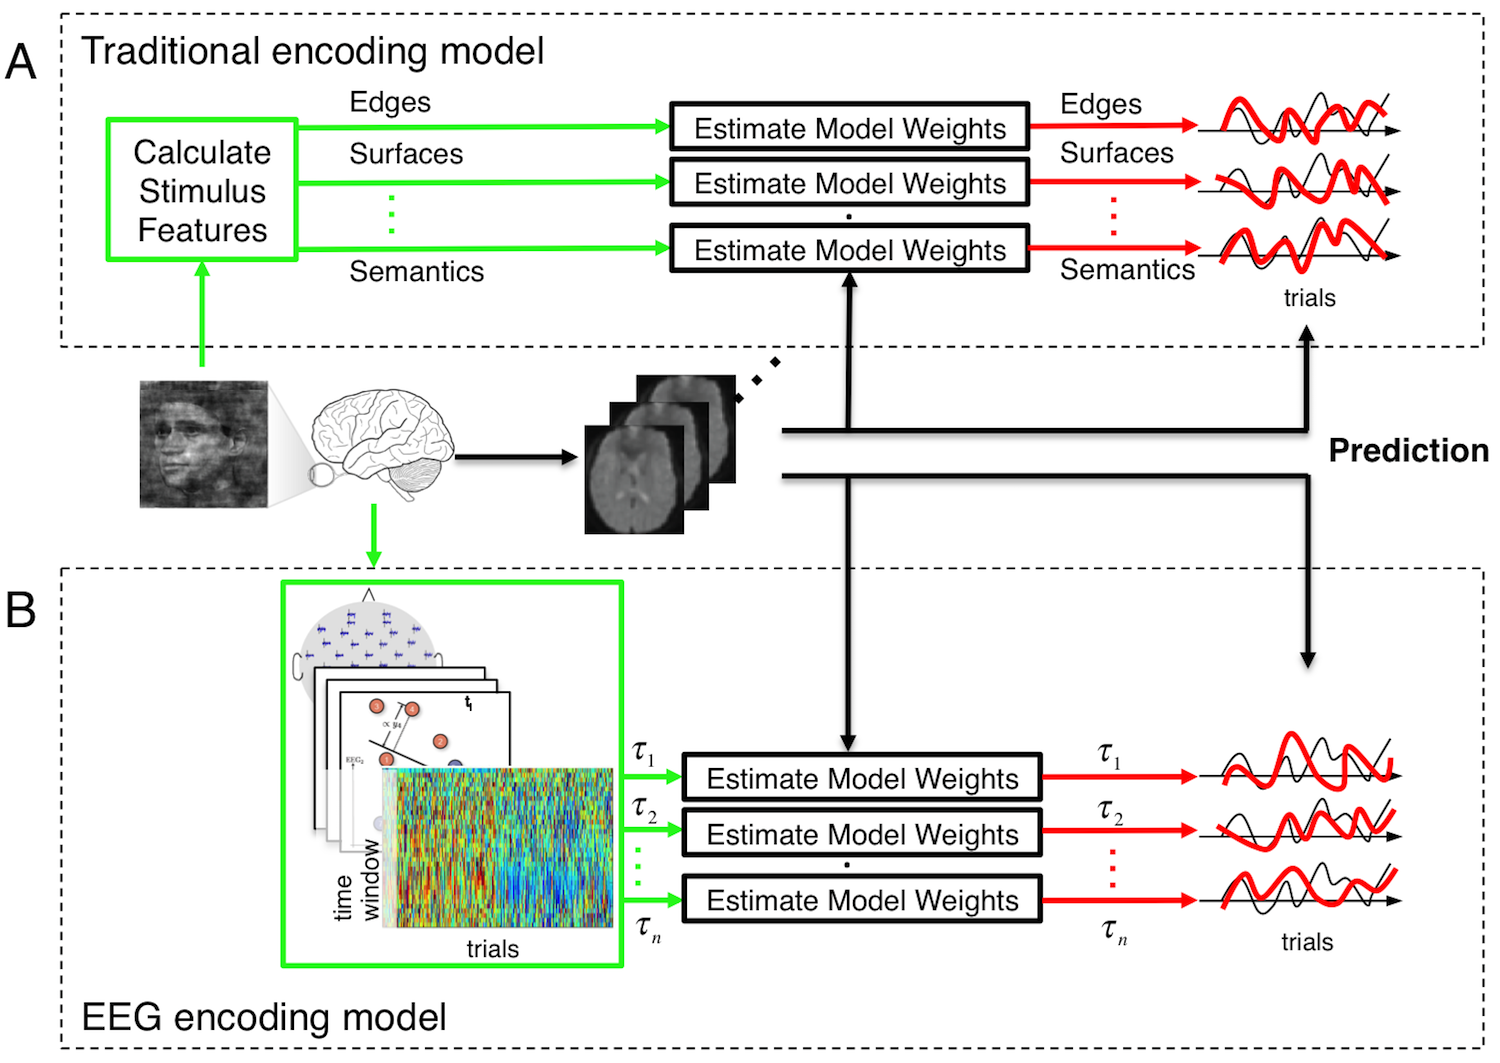
\includegraphics[width=.9\textwidth]{Fig1.png}
\caption{ \textbf{Encoding models based on stimulus derived features versus EEG variability.}\textbf{A}, A traditional encoding model used in fMRI analysis extracts a set of features from the stimulus that are potentially representative of low level structure and high level semantics (green box).  Weights are learned to model how these stimulus features are encoded in the fMRI BOLD signal.  The resulting encoding model is used to make predictions based on how well different voxels predict the features from novel stimuli.  For example, one can create maps of the brain that are labeled based on the stimulus features that each voxel represents. \textbf{B}, The same encoding model concept applied to EEG variability (EEG encoding model).  Instead of features being estimated from the stimulus, they are derived from EEG component trial-to-trial variability (as in Fig 2a) with each temporal window representing a different feature (green box). In traditional encoding models, the stimulus features or concepts are derived through non-linear filters \cite{Cukur2013,Hansen2007,Kay2008,Naselaris2011,Nishimoto2011,Stansbury2013}, however in our model, the non-linearity step is produced by the subject’s brain response to each stimuli which we are able to record with EEG. Weights are learned so as to model how the EEG variability at a given time window is encoded in the fMRI BOLD.  As in the traditional encoding model, predictions on novel stimuli can be done to test the model and results can be used to construct a map —in this case a map of the brain that shows the timing of the EEG component variability that each voxels represents.}
\label{fig:EncodingModel}
\end{figure}

Many previous studies have used known EEG markers (P1, N2, N170, P300, $\alpha$-rhythm) or data driven approaches such as Independent Component Analysis (ICA) to combine EEG with fMRI data \cite{Baumeister2014,DeMartino2010,Huster2012,Jann2009,Jaspers-Fayer2012,Mayhew2013,Nguyen2014,Novitskiy2011,Omata2013,Warbrick2009}. One promising approach has been to use supervised machine-learning techniques (e.g. classifiers) to find relevant projections of the EEG data, where single-trial variability of the electrophysiological response along these projections can be correlated in the fMRI space. Goldman et al.\cite{Goldman2009}, Walz et al.\cite{Walz2013}, Muraskin et al \cite{Muraskin2016}, and Fouragan et al.\cite{Fouragnan2015} have demonstrated this technique on visual and auditory paradigms. This methodology has been shown to localize cortical regions that modulate with the task while preserving the temporal progression of task-relevant neural activity. However, these techniques treat neighboring temporal regions independently when fusing the EEG with fMRI. The approach we present in this paper considers the entire temporal progression of task-specific discriminant activity in the EEG and models how this temporal progression is encoded in the fMRI BOLD data.  Using the full temporal progression allows us to improve temporal resolution and increase the quality of the fit in the encoding model and the accuracy in the subsequent decoding. 

Encoding models have become an important machine learning tool for analysis of fMRI \cite{Naselaris2011}, in that they provide a generative model of the BOLD data (Fig. \ref{fig:EncodingModel}A). In most cases encoding models have been used to learn brain activity that encodes or represents features of a stimulus, such as visual orientation energy in an image/video \cite{Hansen2007,Kay2008,Nishimoto2011}, acoustic spectral power in sound/speech \cite{Silbert2014}, visual imagery during sleep \cite{Horikawa2013} and even high level concepts and semantics \cite{Huth2016}. In the method presented here, however, we employ an encoding model methodology to directly relate the simultaneously collected data from the two neuroimaging modalities. Instead of learning features derived from characteristics of the stimulus, they are derived from the trial-to-trial variability of the EEG components learned via a classifier (Fig. \ref{fig:EncodingModel}B). Specifically, we learn an encoding for the spatially precise fMRI data from the temporally precise trial-to-trial variability of the EEG -- i.e. we learn a mapping that explains the BOLD data given the EEG variability across the time course of each trial. In contrast to previous simultaneous EEG/fMRI techniques that treat the EEG variability at different time points in the trial as independent, we are able to exploit the temporal structure embedded in the EEG by modeling the EEG variability as a time series to accurately predict time course activations in the spatial domain.  

As an example of this method, we apply it to simultaneously acquired EEG/fMRI data collected while subjects performed a perceptual decision-making task. The EEG variability we exploit is derived from a classifier trained to predict the level of stimulus evidence on a trial-to-trial basis from the multichannel EEG data.  This approach leverages the fact that in perceptual decision making tasks, the level of stimulus evidence, as measured via EEG, persists across the trial  \cite{Banko2011a,Philiastides2006}. We can discriminate this information in a time-localized way in the EEG and then temporally ``tag" specific cortical areas by their trial-to-trial variability as they become involved and uninvolved in the decision process. We then proceed to discuss the significance of the results of the new method relative to what can be inferred from non-simultaneously acquired EEG and fMRI.
\section*{Methods}
\subsection*{Subjects}

21 subjects (12 male, 9 female; age range 20-35 years) participated in the study. The Columbia University Institutional Review Board (IRB) approved all experiments and informed consent was obtained before the start of each experiment. All subjects had normal or corrected-to-normal vision.

\subsection*{Stimuli}
We used a set of 30 face (from the Max Planck Institute face database), 30 car, and 30 house (obtained from the web) gray scale images (image size 512x512 pixels, 8 bits/pixel). They all had identical magnitude spectra (average magnitude spectrum of all images in the database) and their corresponding phase spectra were manipulated using the weighted mean phase (WMP) \cite{Dakin2002} technique to generate a set of images characterized by their \% phase coherence. The stimulus evidence (high or low) for each trial was systematically varied by modifying the salience of the image via randomization of image phase at either 35\% (low) or  50\% (high) coherence.

\subsection*{Experimental task}
The stimuli were used in an event-related three-alternative forced choice (3-AFC) visual discrimination task. On each trial, an image — either a face, car, or house — was presented for 50 ms and subjects were instructed to respond with the category of the image by pressing one of three buttons on an MR compatible button controller. Stimuli were presented to subjects using E-Prime software (Psychology Software Tools) and a VisuaStim Digital System (Resonance Technology) with 600x800 goggle display. Images  subtended 11\textdegree x 8\textdegree of visual angle. Over four runs, a total of 720 trials were acquired (240 of each category with 120 high coherence trials) with a random inter-trial interval (ITI) sampled uniformly between 2-4s. Each run lasted for 560 seconds. 

\subsection*{fMRI acquisition}
Blood-oxygenation-level-dependent (BOLD) T2*-weighted functional images were acquired on a 3T Philips Achieva scanner using a gradient-echo echo-planar imaging (EPI) pulse sequence with the following parameters: Repetition time (TR) 2000ms, echo time (TE) 25ms, flip angle 90°, slice thickness 3mm, interslice gap 1mm, in-plane resolution 3x3mm, 27 slices per volume, 280 volumes. For all of the participants, we also acquired a standard T1-weighted structural MRI scan (SPGR, resolution 1x1x1mm). 

\subsection*{EEG acquisition}
We simultaneously and continuously recorded EEG using a custom-built MR-compatible EEG system \cite{Sajda2007,Sajda2010a}, with differential amplifiers and bipolar EEG montage. The caps were configured with 36 Ag/AgCl electrodes including left and right mastoids, arranged as 43 bipolar pairs. Further details are given in Supplementary Material. 

\subsection*{Functional image pre-processing}
Image preprocessing was performed with FSL (www.fmrib.ox.ac.uk/fsl/). Functional images were spatially realigned to the middle image in the times series (motion-correction), corrected for slice time acquisition, spatially smoothed with a 6mm FWHM Gaussian kernel, and high pass filtered (100s). The structural images were segmented (into grey matter, white matter and cerebro-spinal fluid), bias corrected and spatially normalized to the MNI template using ‘FAST’ \cite{Zhang2001a}. Functional images were registered into MNI space using boundary based registration (BBR) \cite{Greve2009}.

\subsection*{EEG data preprocessing}
We performed standard EEG preprocessing offline using MATLAB (MathWorks) with the following digital Butterworth filters: 0.5 Hz high pass to remove direct current drift, 60 and 120 Hz notches to remove electrical line noise and its first harmonic, and 100 Hz low pass to remove high-frequency artifacts not associated with neurophysiological processes. These filters were applied together in the form of a zero-phase finite impulse response filter to avoid distortions caused by phase delays. We extracted stimulus-locked 1500 ms epochs (-500:1000) and subtracted the mean baseline (-200:0) from the rest of the epoch. Through visual inspection, we discarded trials containing motion and/or blink artifacts, evidenced by sudden high-amplitude deflections.

\subsection*{Estimating EEG components and trial-to-trial variability}
We used logistic regression to associate each trial with the level of stimulus evidence represented in the EEG. We considered high stimulus and low stimulus evidence trials irrespective of behavioral accuracy. Regularized logistic regression (r-LR) was used as a classifier to find an optimal projection for discriminating between high and low stimulus evidence trials over a specific temporal window. A sweep of the regularization parameters was implemented using FaSTGLZ \cite{Conroy2013a}. This approach has been previously applied to identify neural components underlying rapid perceptual decision-making \cite{Goldman2009,Muraskin2015,Parra2005,Philiastides2014,Sherwin2012,Sherwin2013,Walz2013,Walz2013a}. 

Specifically, we defined 50ms duration training windows centered at time, $\tau$, ranging from stimulus onset to 800ms following the stimulus in 25ms steps. We used r-LR to estimate a spatial weighting, on all the N EEG channels, that discriminated high stimulus evidence from low stimulus evidence trials. This identifies an Nx1 vector, $w_{\tau}$ , which defines a hyperplane that maximally discriminates between each class (e.g., high vs. low stimulus evidence trials) in the N dimensional space of electrodes. Using this $w_{\tau}$ we calculate the distance each trial is from the decision boundary

\begin{equation}
    y_{\tau}=w^{T}_{\tau}E_{\tau}
\end{equation}

In eqn. 1, $E_{\tau}$ is an N x p vector (N sensors per time window, $\tau$, by p trials). We varied the center of the window ($\tau$) across the trial in 25ms time-steps. For each subject, this produced a matrix $Y$ where the rows corresponded to trials and the columns to training windows, i.e.  $Y$ incorporates the time-window localized trial-to-trial variability in the EEG that we subsequently use to tag the BOLD data. We quantified the performance of the linear discriminator by the area under the receiver operator characteristic (ROC) curve, referred to here as AUC, using a leave-one-out procedure. We used the ROC AUC metric to characterize the discrimination performance at each $\tau$. 

\subsection*{Traditional fMRI analysis}
We first ran a traditional general linear model (GLM) fMRI analysis in FSL, using event-related (high and low stimulus evidence) and response time (RT) variability regressors. Activated regions that passed a family-wise error (FWE) \cite{Nichols2003} corrected cluster threshold of $p < 0.01$ at a z-score threshold of 2.57 were considered significant. Further details can be found in the Supplemental Material. 

\subsection*{fMRI deconvolution}
Associating fMRI data to each trial is challenging for two main reasons: (a) the temporal dynamics of the hemodynamic response function (HRF) evolve over a longer time-scale than the mean ITI of the event-related design, resulting in overlapping responses between adjacent trials; and (b) the ITI was random for each trial so that the fMRI data was not acquired at a common lag relative to stimulus onset. To overcome these issues, we employed the `least squares - separate' (LS-S) deconvolution \cite{Mumford2012} method to estimate the voxel activations for each trial. We extracted 58697 voxels from a common gray matter group mask at $3mm^{3}$ spatial resolution that excluded white matter and CSF and assembled the resulting voxel activations into rows of the data matrix $F$.

\subsection*{Single subject encoding model}
All encoding model analyses were performed in MATLAB. To relate the EEG data with the fMRI, we devised a subject-wise spatiotemporal decomposition using singular value decomposition (SVD). Let F be an m x p matrix denoting m-voxels and p-trials that is the deconvolved high and low stimulus evidence fMRI data for each trial. Let Y be the r x p matrix denoting r-windows (33 $EEG_{\tau}$ windows and response time (RT)) and p-trials. For each trial, the first row of $Y$ is the response times while subsequent rows are the y values at each window time. Let W be an m x r matrix that is the weights on $Y$ that solve for $F$.

\begin{equation}
    F=WY
\end{equation}

Normally, if we solve for $W$ using the least squares approach, we obtain:
\begin{equation}
    W=(FY^{T})(YY^{T})^{-1}	
\end{equation}					

However, each time point might be highly correlated with its neighbors, which reduces the stability of the least-squares regression. We use SVD to reduce the feature space and improve our estimation of $W$ (the weights on each window). For a leave-one-out cross validation, we hold out a single trial from the EEG $Y$ matrix and the corresponding volume from the fMRI data $F$ and train on the remaining trials. We repeated this for all trials. For each leave one out fold we calculated,
\begin{equation}
    Y^{Train}=U \Sigma V^{T}
\end{equation}					
where $U$ is an r x r orthonormal matrix, $\Sigma$ is a r x p diagonal matrix and $V$ is a p x p orthonormal matrix. After SVD on $Y^{Train}$, we reduced the feature dimensions on $Y^{Train}$  to retain 75\% of the variance by only keeping v components. To do this, we selected the first v rows of $\Sigma$ and zeroed the other rows. This results in $\tilde{\Sigma}$  which is our reduced subspace matrix. We recalculate our least squares solution where we have replaced $Y$ by its reduced form $U\tilde{\Sigma}V^{T}$ in equation 3:
 		
\begin{equation}
    \hat{W} = (F^{Train}V\tilde{\Sigma}^{T})(\Sigma\Sigma^{T})^{-1}U^{T}
\end{equation} 				
 			
For each leave one out fold, we first calculated the SVD of the training set. We then calculated the number of components to keep and then solve for $\hat{W}$ , the weight estimate per fold. To test, we applied the weights to the left-out test data $Y^{Test}$ to estimate the encoded fMRI data $\hat{F}$ for the encoding part:

\begin{equation}
    \hat{F}=\hat{W}Y^{Test}
\end{equation}
We constructed the m x r weight matrix $W$ by taking the average of all the trained $\bar{W}$ matrices. For the decoding model we use the left out test data $F^{Test}$ and estimate the EEG variability $\hat{Y}$:
 \begin{equation}
     \hat{Y} = \hat{W}^{T}F^{Test}(\hat{W}^{T}\hat{W})^{+}
 \end{equation}
 Here, $\hat{W}^{T}\hat{W}$ is not invertible, and instead use the pseudo-inverse (denoted by +).
 
Given  $\hat{F}$, an m x p matrix with m voxels by p trials, for each voxel j, we calculated the correlation over trials of $\hat{F_{j}}$ with $F^{Test}_{j}$, resulting in the matrices $R^{fMRI}$ (Pearson Correlation Map) and $P^{fMRI}$  (p-value map of the Pearson Correlation) that are m x 1. The $P^{fMRI}$ was then converted to a z-score map. Thus, we have a map for each subject indicating that subject’s encoding model significance at each voxel. To test which time windows were significant in the decoding model, we also calculated,  $R^{EEG}_{\tau}$ , the correlation between $\hat{Y_{\tau}}$ and $Y_{\tau}$. For each subject, $R^{EEG}_{\tau}$ indicates how well the decoding model predicts EEG variability at each time window from a single fMRI volume. 

% It is important to note that this approach does not attempt to improve source localization typically done for EEG/MEG studies. Our approach instead provides the temporal resolution of EEG (ms) and the spatial resolution of fMRI (mm) without the need to solve the ill-posed inverse solution and make the many associated assumptions required for reliable source-localization results \cite{Wendel2009}.

\subsection*{Group level spatiotemporal analysis}

We evaluated both the encoding model and the resulting decoding model at the group level.  First, to identify group level voxels where our encoding model predictions were consistent across subjects, each subject's p-value maps for the leave-one-out correlation ($R^{fMRI}$) were converted into their respective z-values, then a one-sample t-test testing for the mean difference from 0 was calculated for each voxel and voxel-wise significance was calculated using threshold-free cluster enhancement (TFCE) using a non-parametric randomization procedure implemented in FSL\cite{Smith2009a}. TFCE is an alternative to cluster thresholding in which raw voxel-wise t-statistics are adjusted based on neighboring spatial clusters, producing corrected whole brain volumes. It generally allows for better sensitivity than other thresholding methods. Voxels were considered significant if they passed a false discovery rate (FDR) threshold of p \textless 0.01. 

These significant voxels were then used as a mask to temporally localize weight values in $\hat{W}$  by computing the voxels that were consistent in their direction (positive (high stimulus evidence) or negative (low stimulus evidence)) and timing ($\tau$ window) across subjects. Here, the goal was to develop a statistical parametric map of $\hat{W}$ that identifies significant results in both space and time, thereby creating a spatiotemporal map of a perceptual decision.

First, a one-sample t-test across the subjects’ $\hat{W}$  was computed for all voxels. This generates a statistical parametric map of T-scores in space (voxels) and time (windows). To correct for multiple comparisons, we implemented a spatiotemporal TFCE (stTFCE) in both space (neighboring voxels) and time (neighboring time windows - response time window not included) and computed significance through a randomization procedure. 33000 permutations (1000 permutations per window) were run by randomly altering the sign of the voxel weights from each subject and the temporal ordering of the windows, as we were testing whether the weights were consistent in sign, voxel space, and temporal window. The final statistical parametric map was calculated by comparing the true stTFCE value with the distribution of permuted values for each voxel. Again, voxels were considered significant if they passed FDR correction at p \textless 0.05 (high stimulus evidence: FDR-Corrected p \textless 0.0019, low stimulus evidence: FDR-Corrected p \textless 0.00036). Note that now our number of multiple comparisons was the number of voxels in the FDR-mask (20256) times the number of time windows (33). We analyzed the response time separately with a standard TFCE randomization procedure implemented in FSL.

We also tested the quality of the resulting decoding model at the group level.  To construct group level statistics for the decoding model, we first analyzed the $R^{EEG}_{\tau}$ vectors across all subjects to identify time windows when the model was consistent across subjects. The vectors were converted into their p-values, and for each time window ($\tau$), were used to compute combined Stouffer p-values 45 across all subjects\cite{Darlington2000}. These group level results were then corrected for multiple comparisons using p \textless 0.05 FDR. 

\subsection*{Estimation of subject-trial specific reactivation strength}
As discussed below in Results, we observed a complex time dependence in certain brain regions which appears to be a recapitulation or reactivation of those regions near the end of each trial. In order to estimate the strength of this reactivation we used the encoding model weights ( $\hat{W}$), to estimate the trial-to-trial activation amplitude at different time windows. To specifically estimate the reactivation amplitudes, we took the mean across time of $Y^{R}_{j,i} = W^{T}_{j,PostACC}F_{j,i}$  for each subject (j) and trial (i). Here,$W_{PostACC}$ is the weight matrix from the encoding model restricted to voxels that were significant in the spatiotemporal group results from the 600-800ms windows, i.e. , subsequent to ACC activation (Fig. 6A). By applying the weights restricted to these spatial areas and temporal windows to each trial, we are able to obtain a trial-to-trial value for `reactivation'. $Y^{R}_{j,i}$ was quintiled for high and low stimulus evidence and the average confidence proxy was calculated within each quintile. A linear mixed effects model \cite{Bates2015} was used to test if the slope of confidences across quintile grouping, $Y^{R}_{j,i}$ , was significantly different from 0 while including stimulus evidence as a condition. Separate similar analyses with non-replay windows weights (175-250ms) were also performed. In addition to the confidence proxy analyses, we ran the same linear mixed effects model correlating reactivations with the average behavioral accuracy within each quintile. To test the contribution of each cluster to the correlation with confidence, we implemented recursive feature elimination, where our features were clusters of significant voxels (\textless 48 voxels) during the 600-800ms time window. This procedure removed clusters from the `reactivation' network before calculating trial-to-trial reactivation. We then calculated the percent change in slope (reactivation x confidence proxy; see definition of confidence proxy below) when the cluster was removed compared to the total network. This procedure ranks cluster importance by sorting which clusters, when removed, had the strongest negative effect on slope height.  



%Using the encoding model weights ($\bar{W}$), we are able to estimate the trial-to-trial activation amplitude at different time windows. To estimate the reactivation amplitudes, we took the mean across time of $Y^{R}_{j,i} = W^{T}_{j,PostACC}F_{j,i}$  for each subject (j) and trial (i). Here,$W_{PostACC}$ is the weight matrix from the encoding model restricted to voxels that were significant in the spatiotemporal group results from the 600-800ms windows. By applying the weights restricted to these spatial areas and temporal windows to each trial, we are able to get a trial-to-trial value for ``��reactivation"��. Note that because the reactivation is stronger in the more difficult trials the significant voxels in W are negative and so more negative y's indicate stronger reactivation while more positive y's indicate weaker reactivation.  Separate similar analyses with non-replay windows (175-250ms) and testing for behavioral accuracy were also performed. To test the contribution of each cluster to the correlation with confidence, we implemented recursive feature elimination, where our features were clusters of significant voxels ($> 48$ voxels) during the 600-800ms time window. This procedure removed clusters from the ‘reactivation’ network before calculating trial-to-trial reactivation. We then calculated the percent change in slope (reactivation x confidence proxy) when the cluster was removed compared to the total network. This procedure ranks cluster importance by sorting which clusters, when removed, had the strongest negative effect on slope height.


\subsection*{Drift diffusion model (DDM) and confidence proxy}
To analyze and better interpret our novel finding of a reactivation in the neural cascade (see Results), we used a DDM to estimate a proxy of confidence in the decision for each trial. Recently, Philiastides et al. \cite{Philiastides2014} showed that for conditions in which the boundary does not change, a proxy for decision confidence for each trial (i) can be computed by calculating $1/\sqrt{RT_{i}-T_{non}}$ , where $T_{non}$ is a subject dependent non-decision time fit by the model. Thus, after modeling the DDM process, each trial's (i) confidence proxy (CP) for each subject (j) was computed by $CP_{i,j} = 1/ \sqrt{RT_{i}-T_{non,j}}$  and then z-scored across trials where $T_{non,j}$ was varied for high or low stimulus evidence trials, separately, so that CP was a measure of relative trial confidence within difficulty levels. 

% The DDM models decision-making in two-choice tasks. Here, we treated the decision (correct vs. incorrect) as our two choices. A drift-process accumulates evidence over time until it crosses one of two boundaries (upper or lower) and initiates the corresponding response\cite{Ratcliff2008}. The speed with which the accumulation process approaches one of the two boundaries (a) is called drift-rate (v) and represents the relative evidence for or against a particular response. 

%We used Hierarchical Bayesian estimation of the Drift-Diffusion Model in Python (HDDM) to calculate the drift rate (v), decision boundary (a) and non-decision time $T_{non}$ for each subject \cite{Wiecki2013}. Specifically, we modeled high and low stimulus evidence response time data separately. This was to ensure our confidence proxies were consistent within trial types. We included the response time and whether the subject got the trial correct. HDDM obtains a sequence of samples (i.e., a Markov chain Monte Carlo; MCMC) from the posterior of each parameter in the DDM. In our model, we generated 5000 samples from the posteriors, the first 1000 (burn-in) samples were discarded, and the remaining samples were thinned by 5\%.
%
\section*{Results}
\begin{figure}[htbp!]
\centering
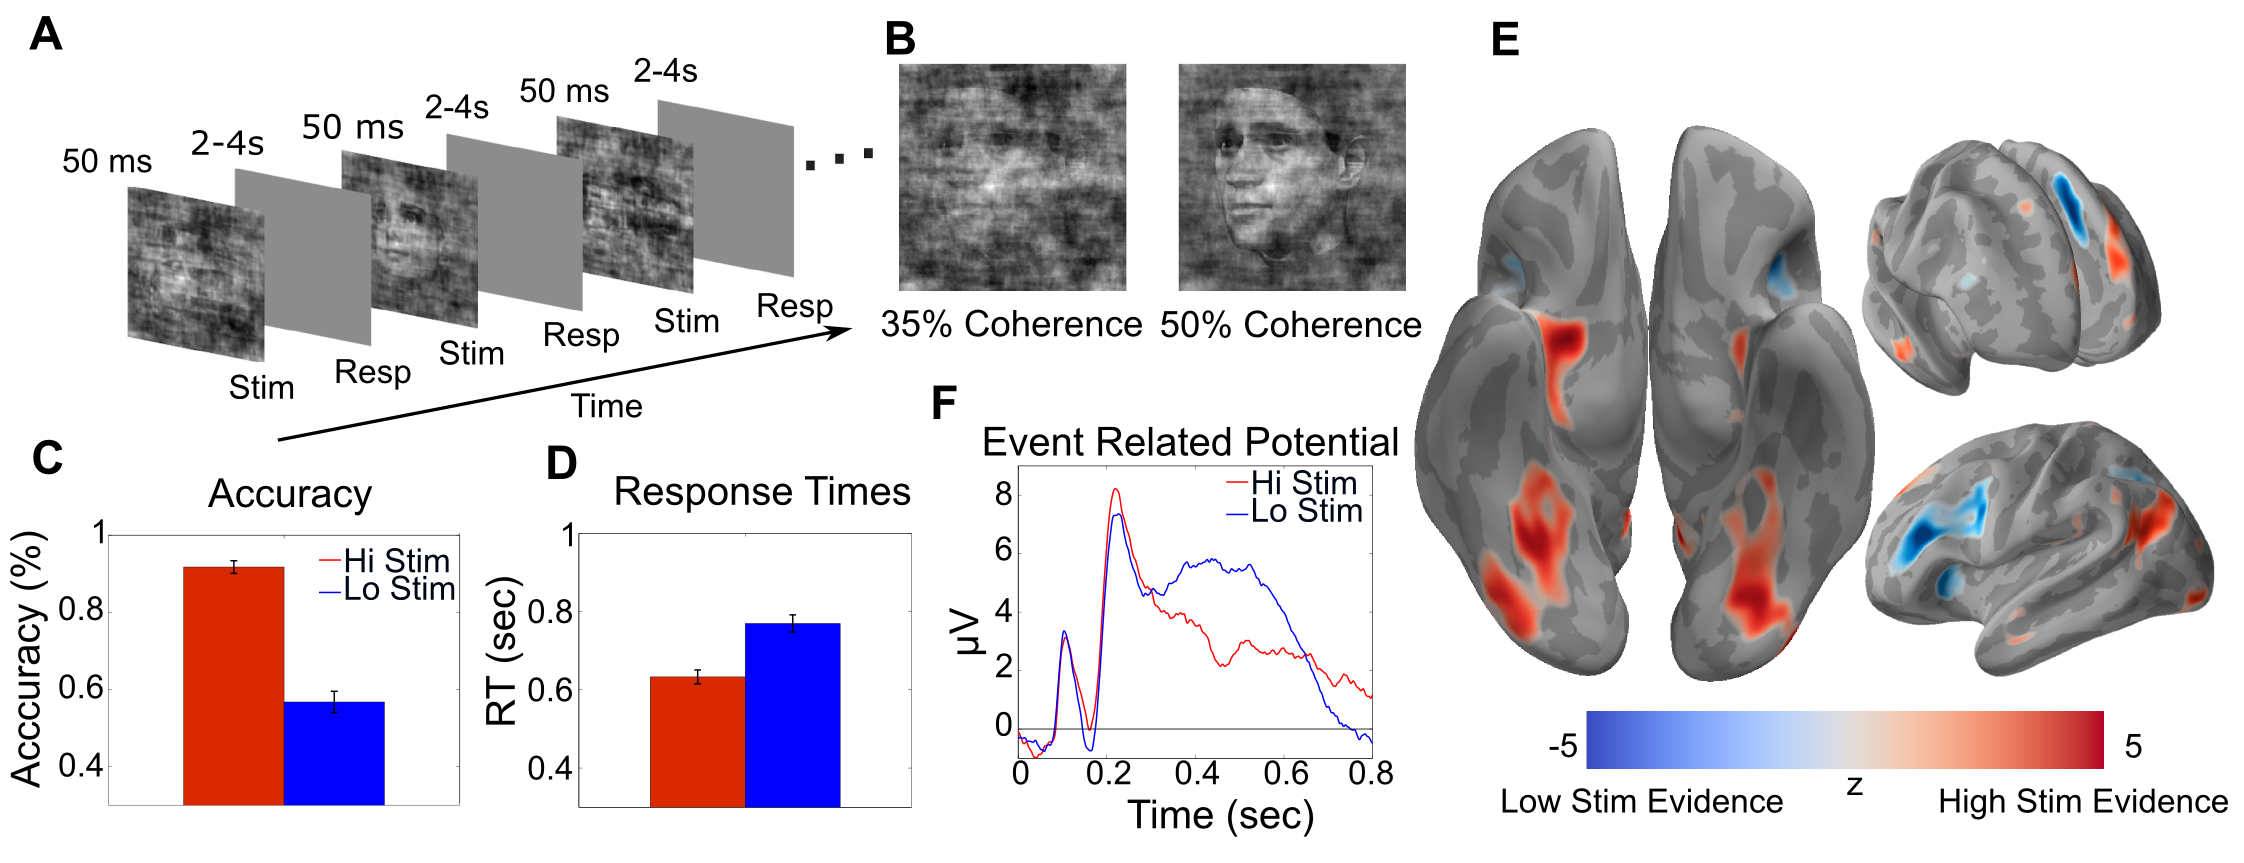
\includegraphics[width=1\textwidth]{Fig2.png}

\caption{ \textbf{Paradigm and traditional EEG and fMRI results.}\textbf{A}, 3-AFC task where stimulus evidence for each category is modulated by varying the phase coherence in the images. \textbf{B}, Example of face images with high stimulus evidence (high  coherence: 50\%) and low stimulus evidence (low coherence: 35\%). \textbf{C}, Behavioral performance shows significant differences, as a function of stimulus evidence, in accuracy ($p< 10^{12}$, paired t-test) and \textbf{D}, response time ($p< 10^{-8}$, paired t-test) across the group. \textbf{E}, fMRI analysis showing cortical areas correlated with high (red) vs. low (blue) stimulus evidence across the entire trial ($Z> 2.57$ with  $p< 0.01$ Family-Wise Error cluster corrected). \textbf{F}, Grand average stimulus-locked event related potentials (ERPs) for electrode Pz show that differences in stimulus evidence span the time from stimulus to response.}
\label{fig:TradResults}
\end{figure}
As a demonstration of how our method for encoding time-localized EEG variability in simultaneously acquired BOLD data can be used to infer neural cascades underlying perception and cognition, we collected EEG/fMRI data from subjects as they performed a 3-AFC task discriminating between faces, cars, and houses (Fig. \ref{fig:TradResults}A). Subjects were instructed to discriminate the object class after briefly viewing an image corrupted by varying levels of noise (Fig. \ref{fig:TradResults}B) and respond by pressing one of three buttons.  Overall, subjects responded with accuracies of 94 $\pm$ 5\% and 58 $\pm$ 12\% and with response times of 634 $\pm$ 82ms and 770 $\pm$ 99ms for high and low stimulus evidence trials, respectively (Fig. \ref{fig:TradResults}C, D). Subject accuracies and response times across stimulus types (faces, cars, houses) for low stimulus evidence trials were similar; however, for high stimulus-evidence trials subject accuracies were higher and response times were shorter for faces than for cars or houses (See Supplemental Information Fig. S1). 

\subsection*{GLM based analysis of BOLD fMRI shows superposition of cortical areas correlated with stimulus evidence}

We first used a traditional general linear model (GLM) analysis of the fMRI (see Methods) to demonstrate how a difference in stimulus evidence is reflected in in the BOLD data (Fig \ref{fig:TradResults}E, SI Table 1). These results become a baseline case we will compare to relative to the additional information that we can obtain using our encoding model for fusing the BOLD and EEG data. Brain regions showing greater BOLD activation to high vs. low stimulus evidence trials included areas associated with early visual perception and the default mode network, such as fusiform gyrus, parahippocampal gyrus, lateral occipital cortex, superior frontal gyrus, and posterior cingulate cortex. Regions with greater BOLD activation to low vs. high stimulus evidence trials included areas in the executive control and difficulty networks, such as dorsal lateral prefrontal cortex, anterior cingulate cortex, intraparietal sulcus, and insula. IImportant to note is that these GLM results, from the same fMRI data acquired simultaneously with EEG, reproduced previous results in the literature for fMRI collected alone \cite{Heekeren2004}(Fig. S2A) and and can be compared to our results below, thus highlighting that temporal superposition of activations seen in the GLM can be separated in time using our method.

\subsection*{Extracting temporally localized EEG signatures of stimulus evidence variability}

The traditional fMRI results showed multiple brain regions correlated with the stimulus evidence of the trial; however, this traditional approach does not enable one to infer the relative timing of these fMRI activations. From the averaged event related potentials, however, we see that the difference in stimulus evidence (high vs. low stimulus evidence) spans the trial (see Fig \ref{fig:TradResults}F). To infer timing at a scale of tens of milliseconds, we exploit this difference and use linear classification \cite{Parra2005,Sajda2009} of the multichannel EEG to estimate EEG components selective to the trial-to-trial variability in the stimulus evidence.  Importantly these components were estimated at 25ms steps, locked to either the onset of the stimulus or response, so as to encode the BOLD activity at specified time points in the trial.  
\begin{figure}[tb!]
\centering
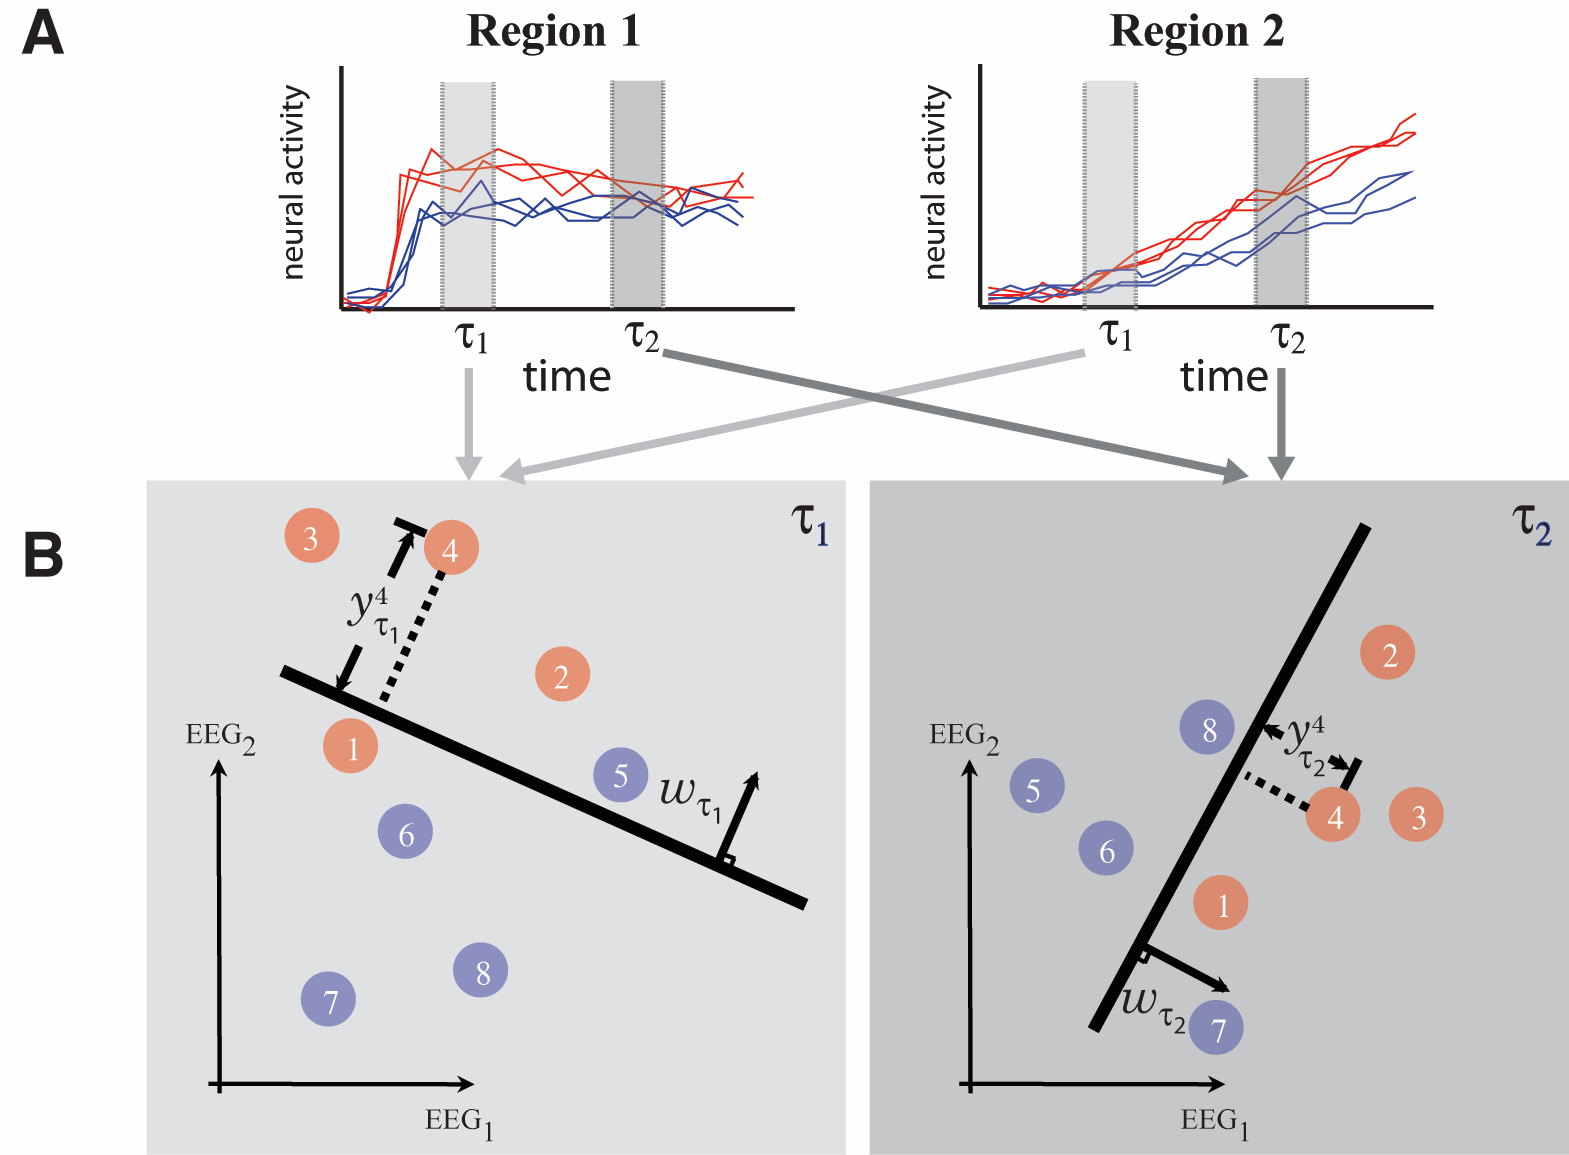
\includegraphics[width=.6\textwidth]{Fig3.png}
\caption{\textbf{Temporally precise trial-to-trial EEG variability tags brain regions during decision-making.}
\textbf{A}, Illustration of how trial-to-trial variability of neural activity in spatially distinct cortical areas can be used to tag brain regions. In this hypothetical example Region 1 is involved in sensory encoding while Region 2 integrates sensory evidence to form a decision (in NHP literature, Region 1 might represent MT, while Region 2 LIP). Neural activity across the trial is shown for two stimulus types, one with high sensory evidence for the choice (red curves) and one with low sensory evidence (blue curves).Also shown are two temporal windows ($\tau_{1}$ and $\tau_{2}$) that represent different times during the trial. \textbf{B}, Linear classifiers are trained to separate trials based on the two levels of stimulus evidence at specific temporal windows.  Shown are classifiers (parameterized by weight vectors $w_{1}$ and $w_{2}$) for two temporal windows ($\tau_{1}$ and $\tau_{2}$) with respect to two EEG sensors (for simplicity only two dimensions of the full N=43 sensor space are shown.  Though the component hyperplane is optimal for the full 43 dimensions, when projected to a line in two dimensions for illustration, it may appear that the separation is sub-optimal). This yields an EEG discriminant component for each temporal window. Variability along these components serves as a unique feature vector for temporally tagging the BOLD data—e.g. variability along an EEG component trained with data from $\tau_{1}$ tags BOLD voxels with time $\tau_{1}$ while variability along an EEG component trained with data from $\tau_{2}$ tags them with $\tau_{2}$.}
\label{fig:variability}
\end{figure}

The basic idea is illustrated in Figure \ref{fig:variability}, where hypothetical neural activity is shown for two different regions that are constituents of the perceptual decision-making network. Averaging over trials would clearly reveal a difference in the mean neural activity between high and low stimulus evidence (as we see in Fig \ref{fig:TradResults}F). However, the two regions contribute differentially to the network, with one region encoding the stimulus evidence (Region 1) and the other integrating it over time (Region 2); both are sensitive to the level of stimulus evidence, though varyingly so at different times in the trial.  By taking advantage of this sensitivity to the stimulus evidence, we can learn EEG discriminant components, i.e. spatial filters, that best classify trials at different time windows given the neural data.  We used the trial-to-trial variability along these component directions as features to uniquely tag fMRI voxels with the specific time window of the component. This tagging is done by building an encoding model of the features, given the BOLD signal, details of which are described in the following section.

We estimated the EEG components by learning linear classifiers at 25ms steps, starting from stimulus onset to 50ms past the average low stimulus evidence response time (800ms).  We chose a time step of 25ms due to an empirical analysis showing a half width of 50ms in the temporal autocorrelation of the EEG data, though in principle this methodology allows for temporal resolution up to the EEG sampling rate. Each classifier was associated with a set of discriminant values, which can be represented as a vector $y_{\tau}$; each element of the vector is the distance of a given trial to the discrimination boundary for the classifier at time step $\tau$ (Fig. \ref{fig:variability}). This distance can be interpreted as a measure of the EEG classifier's estimate of the level of stimulus evidence for that trial \cite{Goldman2009,Muraskin2015,Parra2005,Sajda2009,Sherwin2012,Walz2013}.

Results of the EEG analysis show discriminating information for stimulus evidence spanning the trial (see Fig. \ref{fig:EEGResults}A), beginning roughly 175ms post-stimulus to past the average response times.  A dip occurs around 300ms, indicating stimulus evidence is less discriminative at this time and serves to demarcate early and late cognitive processes. The early process corresponded to the time of the D220 ERP component, which has been shown to modulate with the degree of task difficulty, whether via stimulus noise or task demands \cite{Philiastides2006}. The later and more prolonged component is likely related to more complex cognitive and motor preparatory processes that differ between high and low stimulus evidence trials.  Importantly, although the early and late EEG components were both discriminative, we found their trial-to-trial variability to be uncorrelated (Figs. \ref{fig:EEGResults}B and S3E), indicating that while the discriminating information (level of stimulus evidence) persists across the trial, it couples differently to processes across time. 

\begin{figure}[h!]
\centering
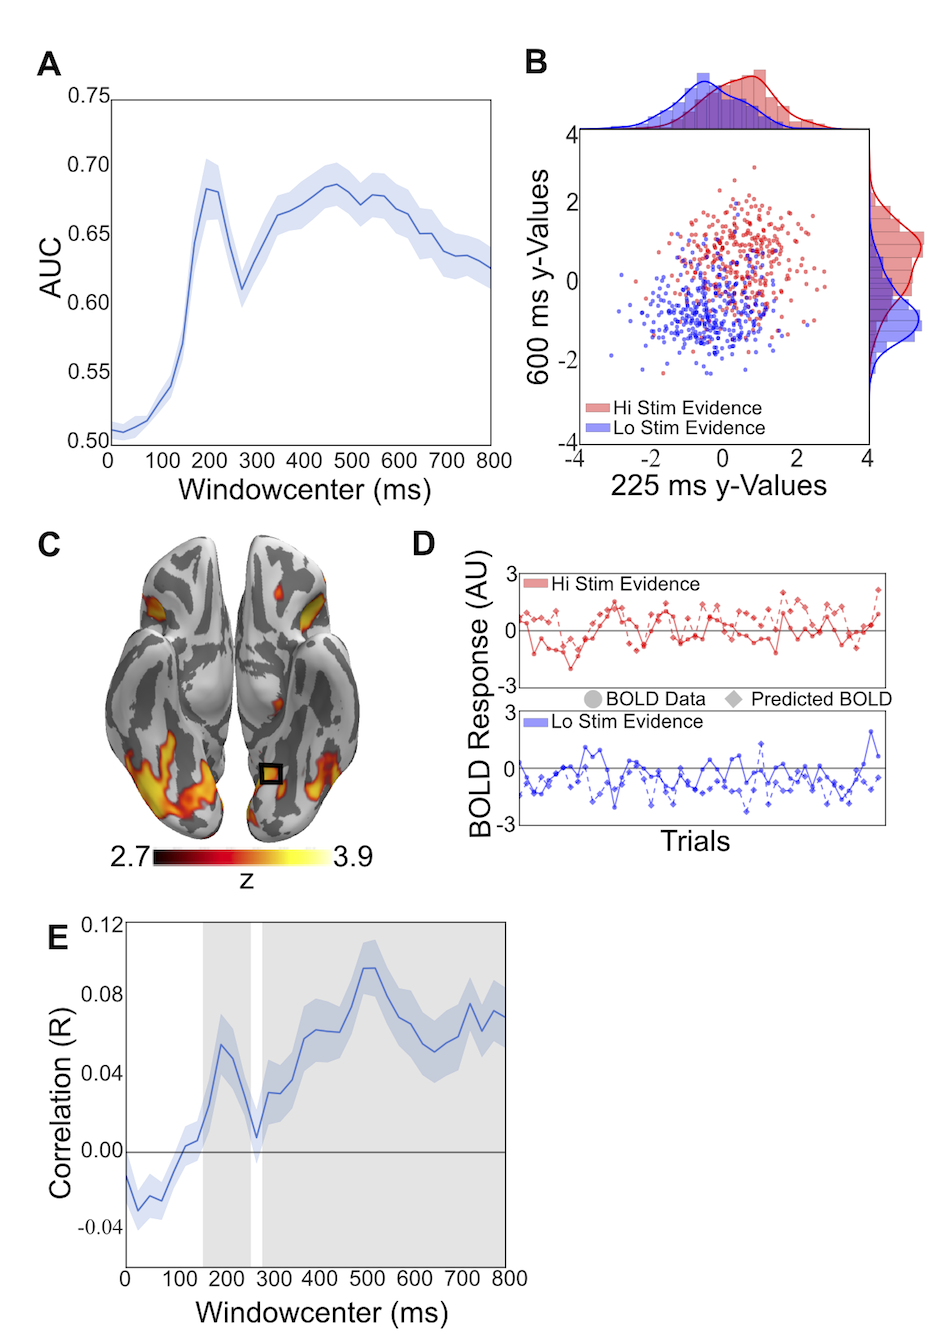
\includegraphics[width=.4\textwidth]{Fig4.png}

\caption{\textbf{EEG discrimination and encoding model results.}\textbf{A}, Group average area under the receiver operating curve (AUC) for the sliding window logistic regression EEG discrimination analysis, comparing high versus low stimulus evidence trials; standard error across subjects is shown with shading. \textbf{B}, A single subject's discriminating y-value distributions for high (red) and low stimulus evidence (blue) trials for two EEG time points (225ms and 600ms). \textbf{C}, Significant fMRI voxels resulting from the group level analysis for the encoding model ($p< 0.01$ TFCE-False Discovery Rate (FDR) corrected). Activity is seen encompassing early visual processing regions, attention networks, and the task positive network. \textbf{D}, A random subset of 100 (50 for each stimulus evidence condition) from 700 total trials of the actual (circle) and predicted (diamond) BOLD responses from the encoding model, for an example subject at a single voxel (MNI X/Y/Z mm: -27/-54/-15, r=0.206, $p<10^{-6}$). High and low stimulus evidence trials are shown separately for clarity. \textbf{E}, The averaged correlation of the predicted y-values with the true y-values across the trial duration. Blue shading represents the standard error across subjects. Grey shading indicates significant time windows ($p< 0.05$ FDR-corrected).}
\label{fig:EEGResults}
\end{figure}

\subsection*{Using an encoding model to link fMRI activations with temporally distinct EEG trial-to-trial variability}

We create feature vectors $y_{\tau}$ by extracting the trial-to-trial variability from the EEG discriminant components across time steps, $\tau$, along with a response time vector to construct a matrix $Y$.  This matrix is the temporally precise representation of the trial-to-trial EEG variability that reflects high vs. low stimulus evidence. An encoding model (see Methods) is then fit to predict the trial-to-trial variability of the BOLD response for each fMRI voxel. The model can be seen as  ``taging" each voxel with a ``time", or set of times, when it encodes the variability in the given EEG discriminant component(s).

The group level result of the encoding model is shown in Fig. \ref{fig:EEGResults}C (see also Fig. S2B) where significant voxels from the encoding model are shown in yellow. Fig. \ref{fig:EEGResults}D shows the trial-to-trial variability of BOLD signal at a specific voxel, comparing it to the variability predicted by the encoding model. Additional validity of the encoding model and single subject results are presented in the Supplemental Information (Fig. S4A/B). The encoding model was also evaluated as a decoding model (see Methods) with the BOLD activity used to predict the trial-to-trial variability in the EEG for unseen data--data on which the encoding model was not trained. Fig. \ref{fig:EEGResults}E shows these results, expressed as the correlation between the measured and predicted EEG trial-to-trial variability across the 800ms epoch. The shape of the curve is highly consistent with that observed for the EEG data itself (comparing Fig. \ref{fig:EEGResults}A and Fig. \ref{fig:EEGResults}E) (additional analysis of the fidelity of the model is provided in the SI, Fig. S3).


\begin{figure}[htb!]
\centering
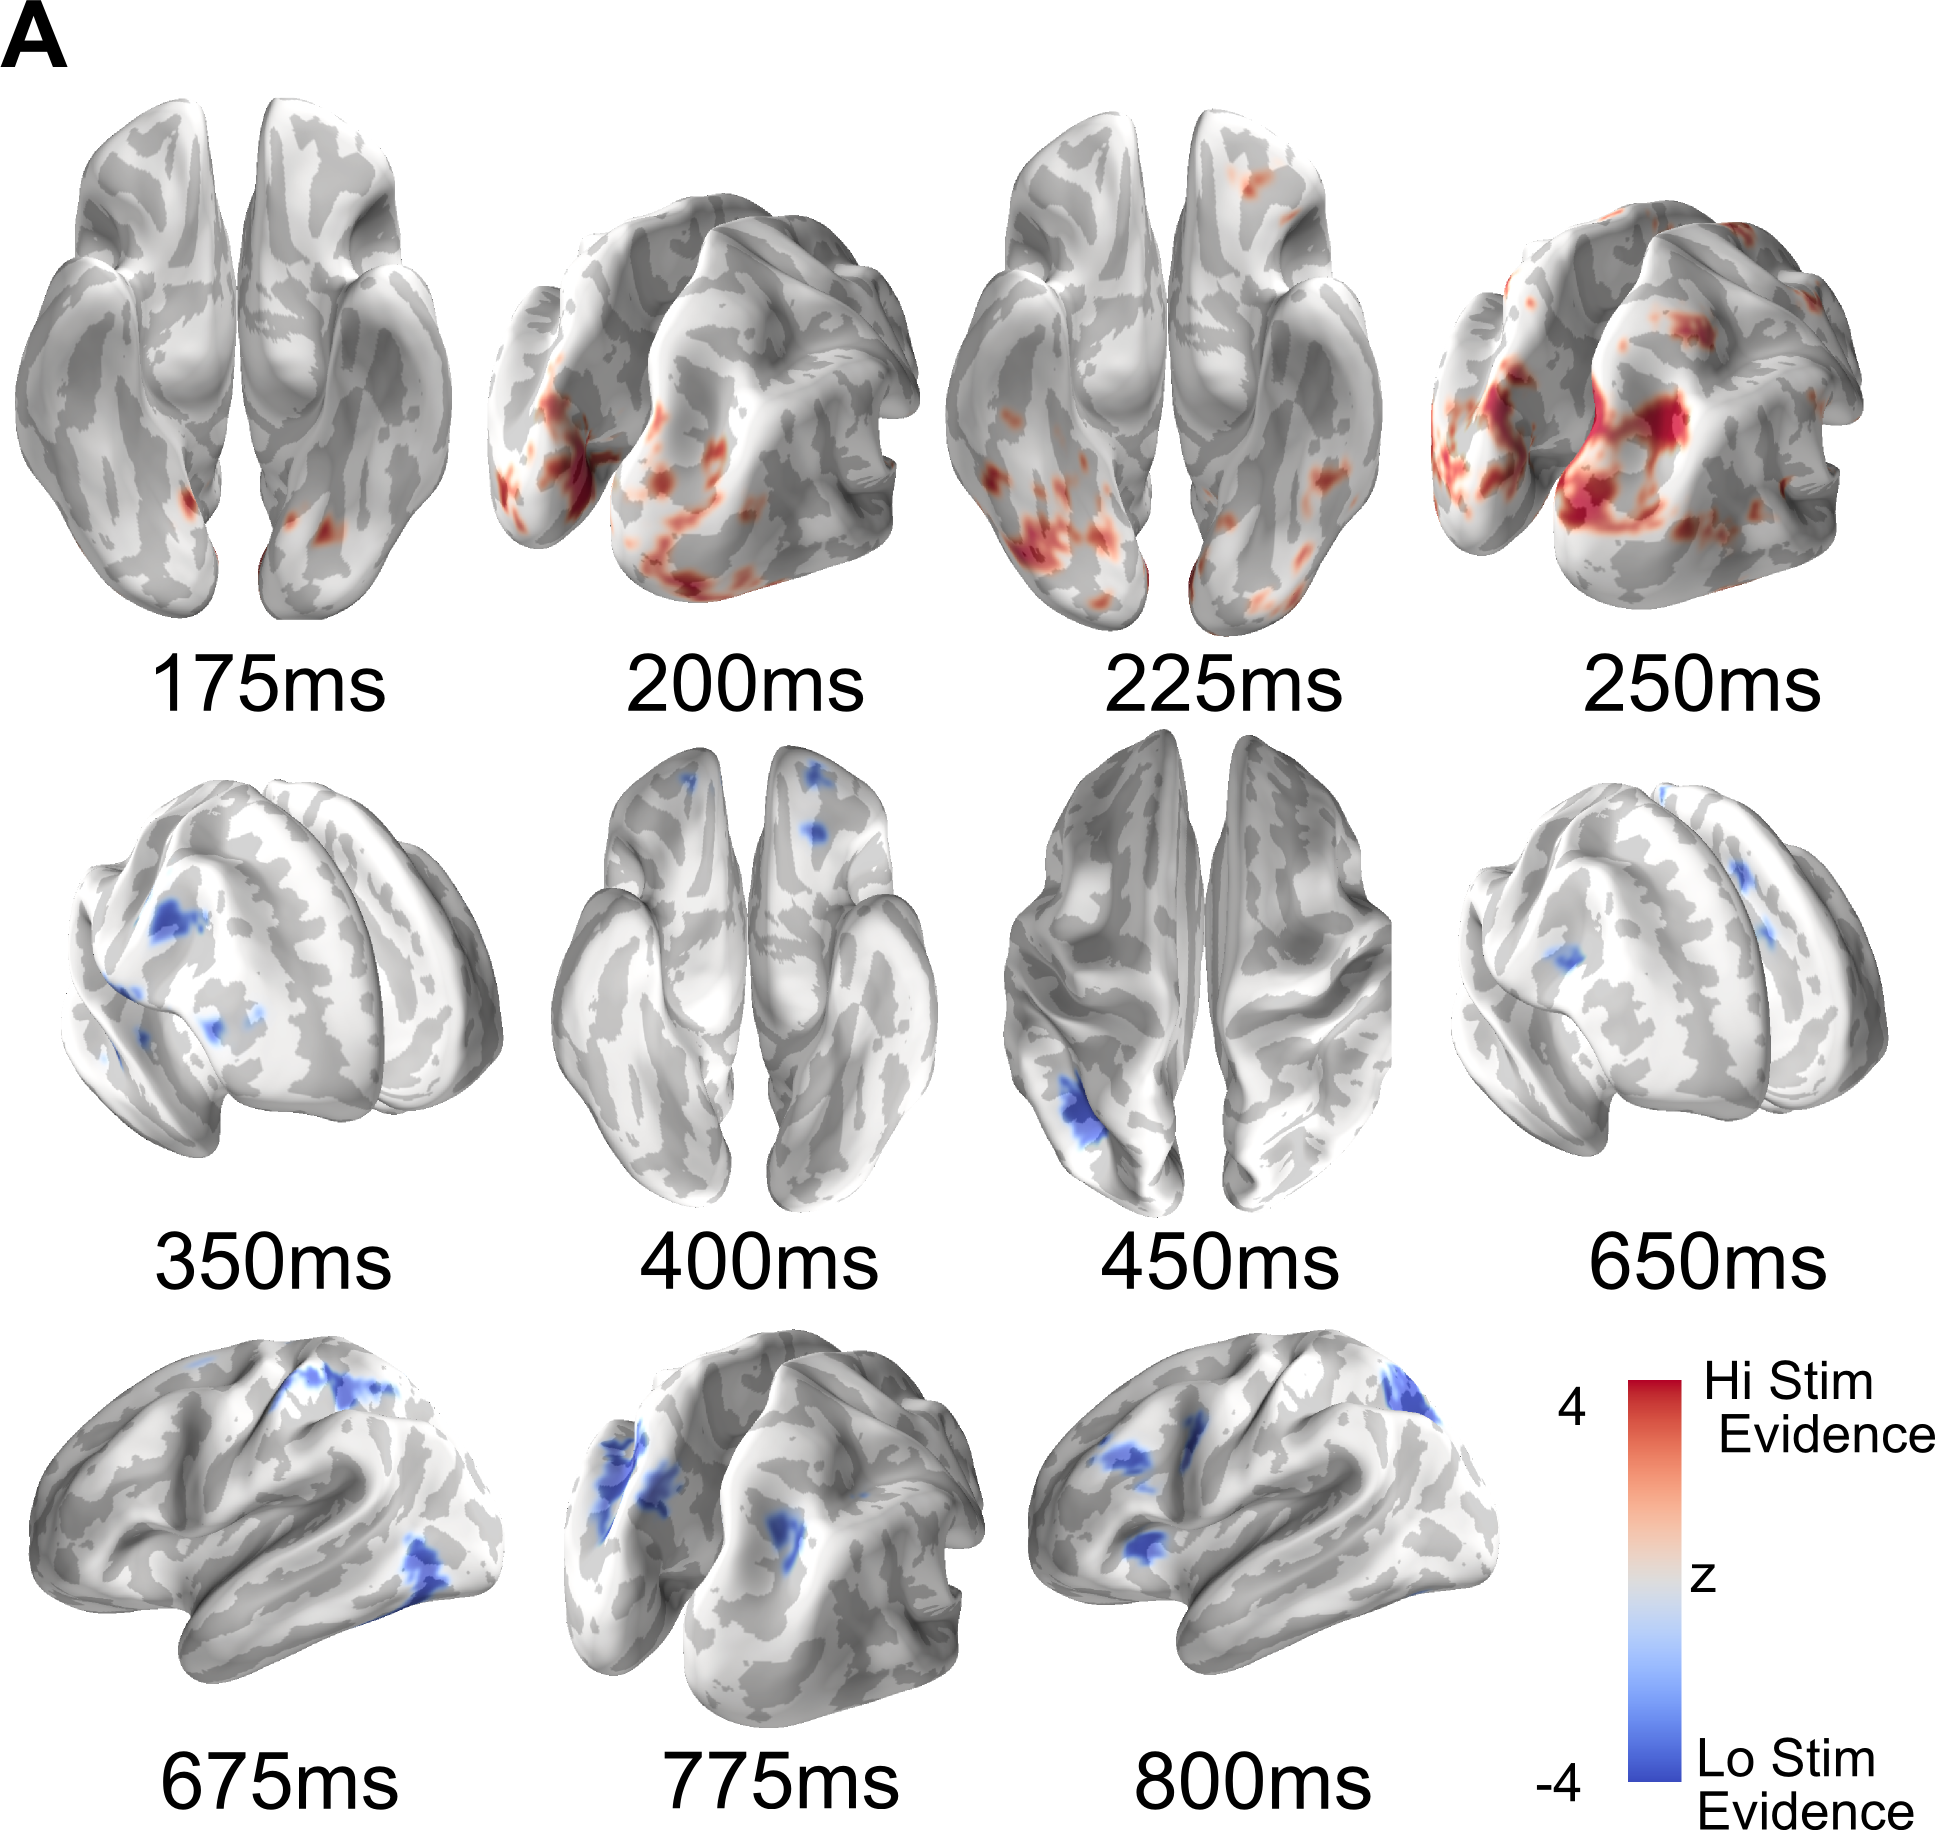
\includegraphics[width=.5\textwidth]{Fig5.png}
\caption{\textbf{Group-level encoding model weights results show neural activation cascade}. Subset of thresholded ($p< 0.05$ FDR-Corrected, k=10) group level statistical parametric maps created by stTFCE randomization procedure on the encoding model weight matrices show the progression of spatial activity across the trial. Activation can be seen early in the trial in the occipital regions while progressing more anteriorly later in the trial to executive control areas. Activations in red indicate areas where high stimulus evidence trials had larger activations than low stimulus evidence trials, and blue the inverse.}
\label{fig:fMRIResults}
\end{figure}

Given the encoding model, we construct the progression of the BOLD activity across time by identifying voxel weights that are consistent across subjects in space and time (see Methods). Fig. \ref{fig:fMRIResults} shows the significant voxel locations in the spatio-temporal statistical parametric maps for the group level analysis. The weights from the encoding model can be interpreted similarly to the Beta-weights in a traditional GLM contrast. Here, red voxels indicate significant regions where EEG discrimination y-values for high stimulus evidence positively covary with BOLD signal, and blue voxels indicate a negative covariation between more negative (low evidence) EEG discrimination y-values and BOLD signal. We observe a progression of activity (see also Movie S1), at 25ms resolution, which proceeds simultaneously down the dorsal and ventral streams of visual processing for the first 250ms. After that the cascade becomes more complex with activation in the IPS at 425ms and 750ms (see Fig. \ref{fig:EncodingResults}A), reactivation of the SPL at 675ms and activation of ACC at 600ms along with other regions found in the traditional fMRI results. (see Tables S2). The reactivation pattern is particularly significant since it would not be observable via a traditional fMRI general linear model (GLM) analysis (results of which were presented in Fig. \ref{fig:TradResults}E), which integrates over time and thus superimposes these activities. For example, the changing sign of the middle temporal gyrus (MT) encoding weights in Fig. \ref{fig:EncodingResults}A manifested as no activity in the MT for the traditional fMRI GLM analysis using this same BOLD data--the change in sign canceled the effective correlation in the GLM. The areas of activation we find are internally consistent with the traditional GLM results (see Fig. S2E/F) and with previous reports in the literature for human subjects\cite{Heekeren2004,Philiastides2007}; however, here we are able to link activations across time in a way that was previously only possible with invasive techniques. 

%Given the encoding model, we construct the progression of the BOLD activity across time by identifying voxel weights that are consistent across subjects in space and time (see Methods). Fig. \ref{fig:fMRIResults} shows these results for a group level analysis. The weights from the encoding model can be interpreted similarly to the $\beta$-weights in a traditional GLM contrast. Here, red voxels indicate significant regions where high stimulus evidence variability positively covary between EEG discrimination y-values and BOLD activation and where blue voxels indicate a negative covariation between more negative EEG discrimination y-values (stronger low evidence discrimination) and BOLD activation. We observe a progression of activity (see also Movie S1), at 25ms resolution, which proceeds simultaneously down the dorsal and ventral streams of visual processing for the first 250ms. After that the cascade becomes more complex with activation in the IPS at 425ms and 750ms (see Fig. \ref{fig:EncodingResults}A), reactivation of the SPL at 675ms and activation of ACC at 600ms along with other regions found in the traditional fMRI results. (see Tables S2). The reactivation pattern is particularly significant since it would not be observable via a traditional fMRI general linear model (GLM) analysis (results of which were presented in Fig. \ref{fig:TradResults}E), which integrates over time and thus superimposes these activities. For example, the changing sign of the middle temporal gyrus (MT) encoding weights in Fig. \ref{fig:EncodingResults}A manifested as no activity in the MT for the traditional fMRI GLM analysis of this same BOLD data--the change in sign canceled the effective correlation in the GLM. The areas of activation we find are internally consistent with the traditional GLM results (see Fig. S2E/F) and with previous reports in the literature for human subjects \cite{Heekeren2004,Philiastides2007}; however, here we are able to link activations across time in a way that was previously only possible with invasive techniques. 

\begin{figure}[htb!]
\centering
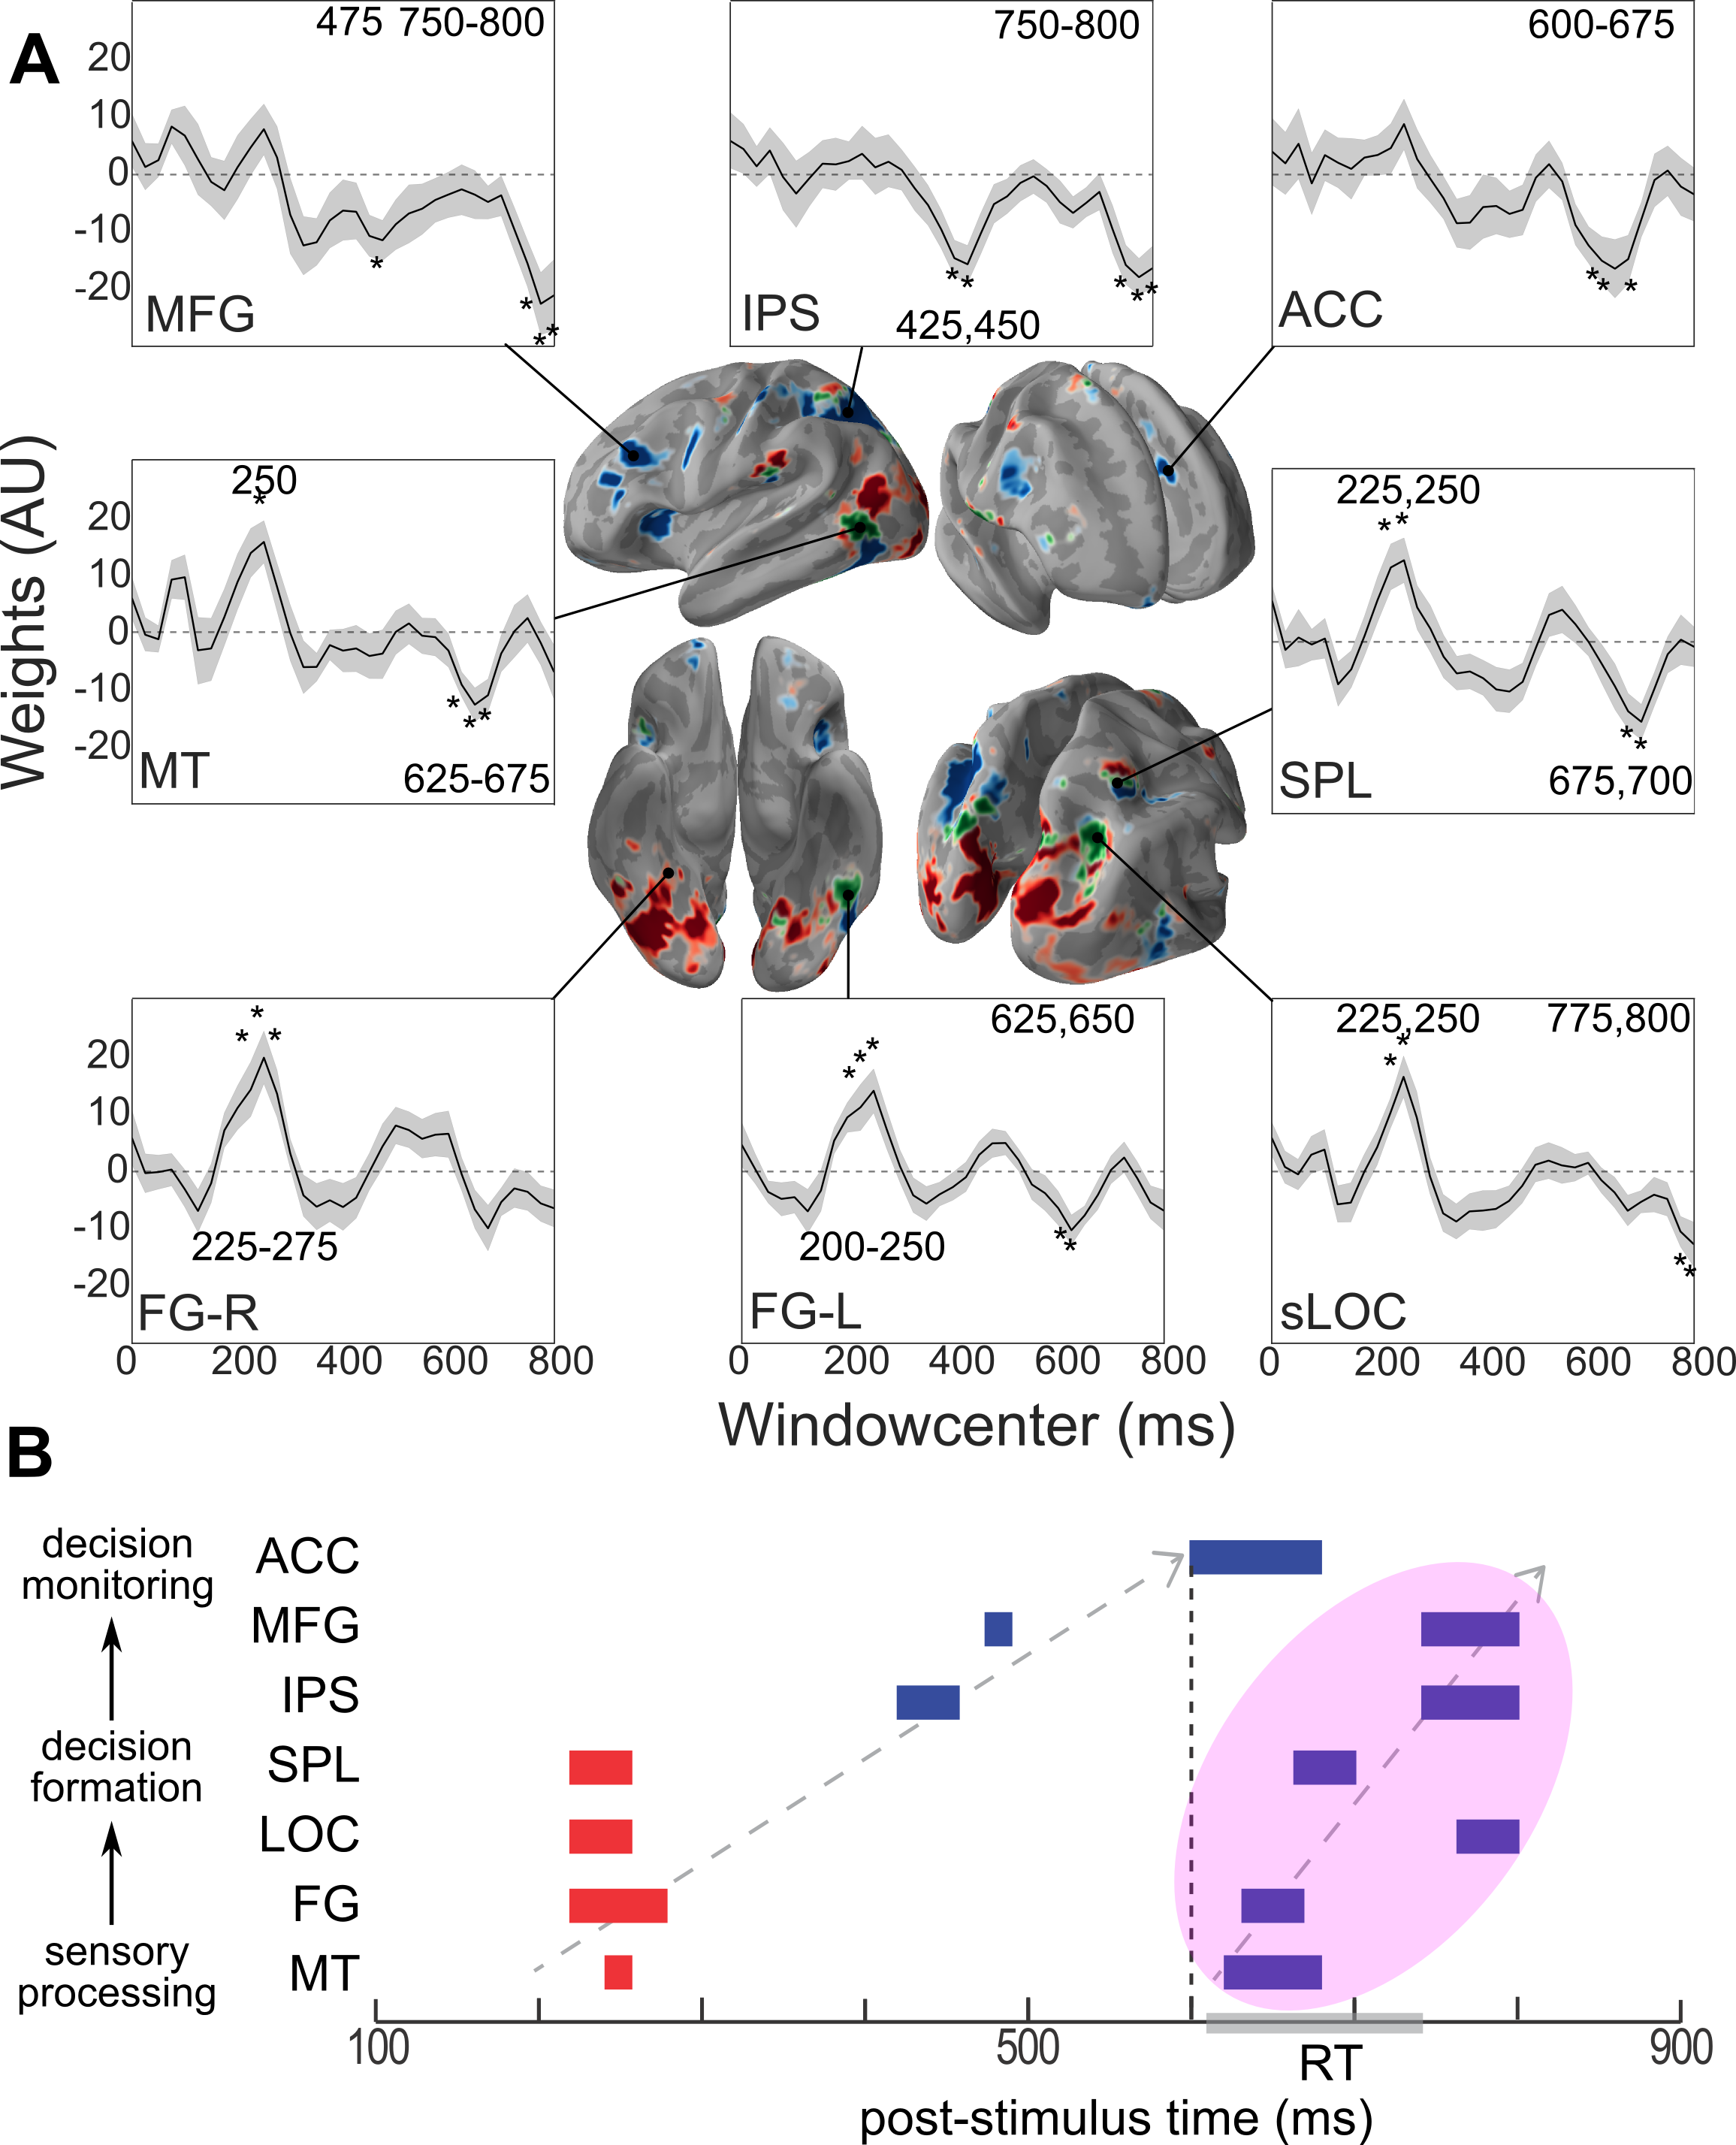
\includegraphics[width=.6\textwidth]{Fig6.png}
\caption{\textbf{Spatial-temporal event-related activations show coordinated reactivations.}\textbf{A}, Union across time windows of significant voxels for high (red) and low (blue) stimulus evidence activations. Voxels with activations for both high and low conditions (at different time windows) are displayed in green (Fig. S2C). Also shown are the encoding model weights for specific voxels, including fusiform gyrus (FG-R):36/-51/-18, (FG-L):-42/-42/-18, superior lateral occipital cortex (sLOC):24/-63/36, superior parietal lobule (SPL):27/-51/54, anterior cingulate cortex (ACC):-6/24/30, intraparietal sulcus (IPS):-30/-60/39, middle frontal gyrus (MFG):-45/27/30, middle temporal gyrus (MT):-57/-60/0. Asterisks indicate significant windows. \textbf{B}, Sequence of significant weights showing a ``replay" of the network after the onset of ACC activation (shaded ellipse). ``Replay" is faster than the initial stimulus driven sequence and strongest for low evidence trials.}
\label{fig:EncodingResults}
\end{figure}

\subsection*{Cortical reactivation correlates with decision confidence}

We identified a reactivation pattern in the spatiotemporal dynamics which was not observable using non-simultaneously acquired EEG or fMRI. Further analysis of the spatiotemporal dynamics (see Fig. \ref{fig:EncodingResults}B) shows that the reactivation pattern in the network occurs after decision-monitoring areas become engaged (i.e. after activation of ACC). Spontaneous reactivation, or ``replay," of neural activity in the human brain has been observed and is believed to be important for memory consolidation \cite{Deuker2013} and more recently has been hypothesized to play a role in perceptual decision-making by enabling the formation of decision confidence \cite{Fleming2012}. To test the hypothesis that the reactivation activity we see may be related to decision confidence, we used a hierarchical drift diffusion model (DDM) \cite{Ratcliff2008,Wiecki2013} to fit the behavioral data for high and low stimulus evidence conditions (see Methods).  Specifically, our model enables us to define a proxy for decision confidence based on the DDM fits to the behavior \cite{Kiani2014,Philiastides2014}. 

Correlating the reactivation level to this confidence proxy shows a strong and significant monotonic relationship between confidence proxy and the level of reactivation (high stimulus evidence-slope=0.037$\pm$0.008, t=4.657, $p=3.2x10^{-6}$; low stimulus evidence-slope=0.062$\pm$0.008, t=7.754, $p=8.88x10^{-15}$), with low stimulus evidence trials reactivated more strongly than high stimulus evidence trials (difference in slopes=-0.025$\pm$0.011, t=2.189, p=0.029)(see Fig. \ref{fig:Confidence} and Fig. S5a). Additionally, reactivation amplitude correlates with behavioral accuracy (Fig. S5b) (high stimulus evidence, slope=0.0115$\pm$0.0047, t=2.41, p=0.016; low stimulus evidence, slope=0.0104$\pm$0.0047, t=2.19, p=0.028).  Additional control analyses from early time windows (175-250ms) shows no significant correlations between activation and confidence proxy (Fig. S5).

We next analyzed which cortical regions most contributed to this reactivation. Specifically, we used a recursive feature elimination to identify those regions contributing the most to the correlation between the level of reactivation and the confidence proxy.  We found that the IPS/SPL and dorsal lateral prefrontal cortex (DLPFC) contributed the most (Fig. \ref{fig:Confidence}C). Interestingly, these two areas have been previously implicated in metacognitive judgments of confidence \cite{Fleming2012,Steinhauser2010,Yeung2012}.

\begin{figure}[htb!]
\centering
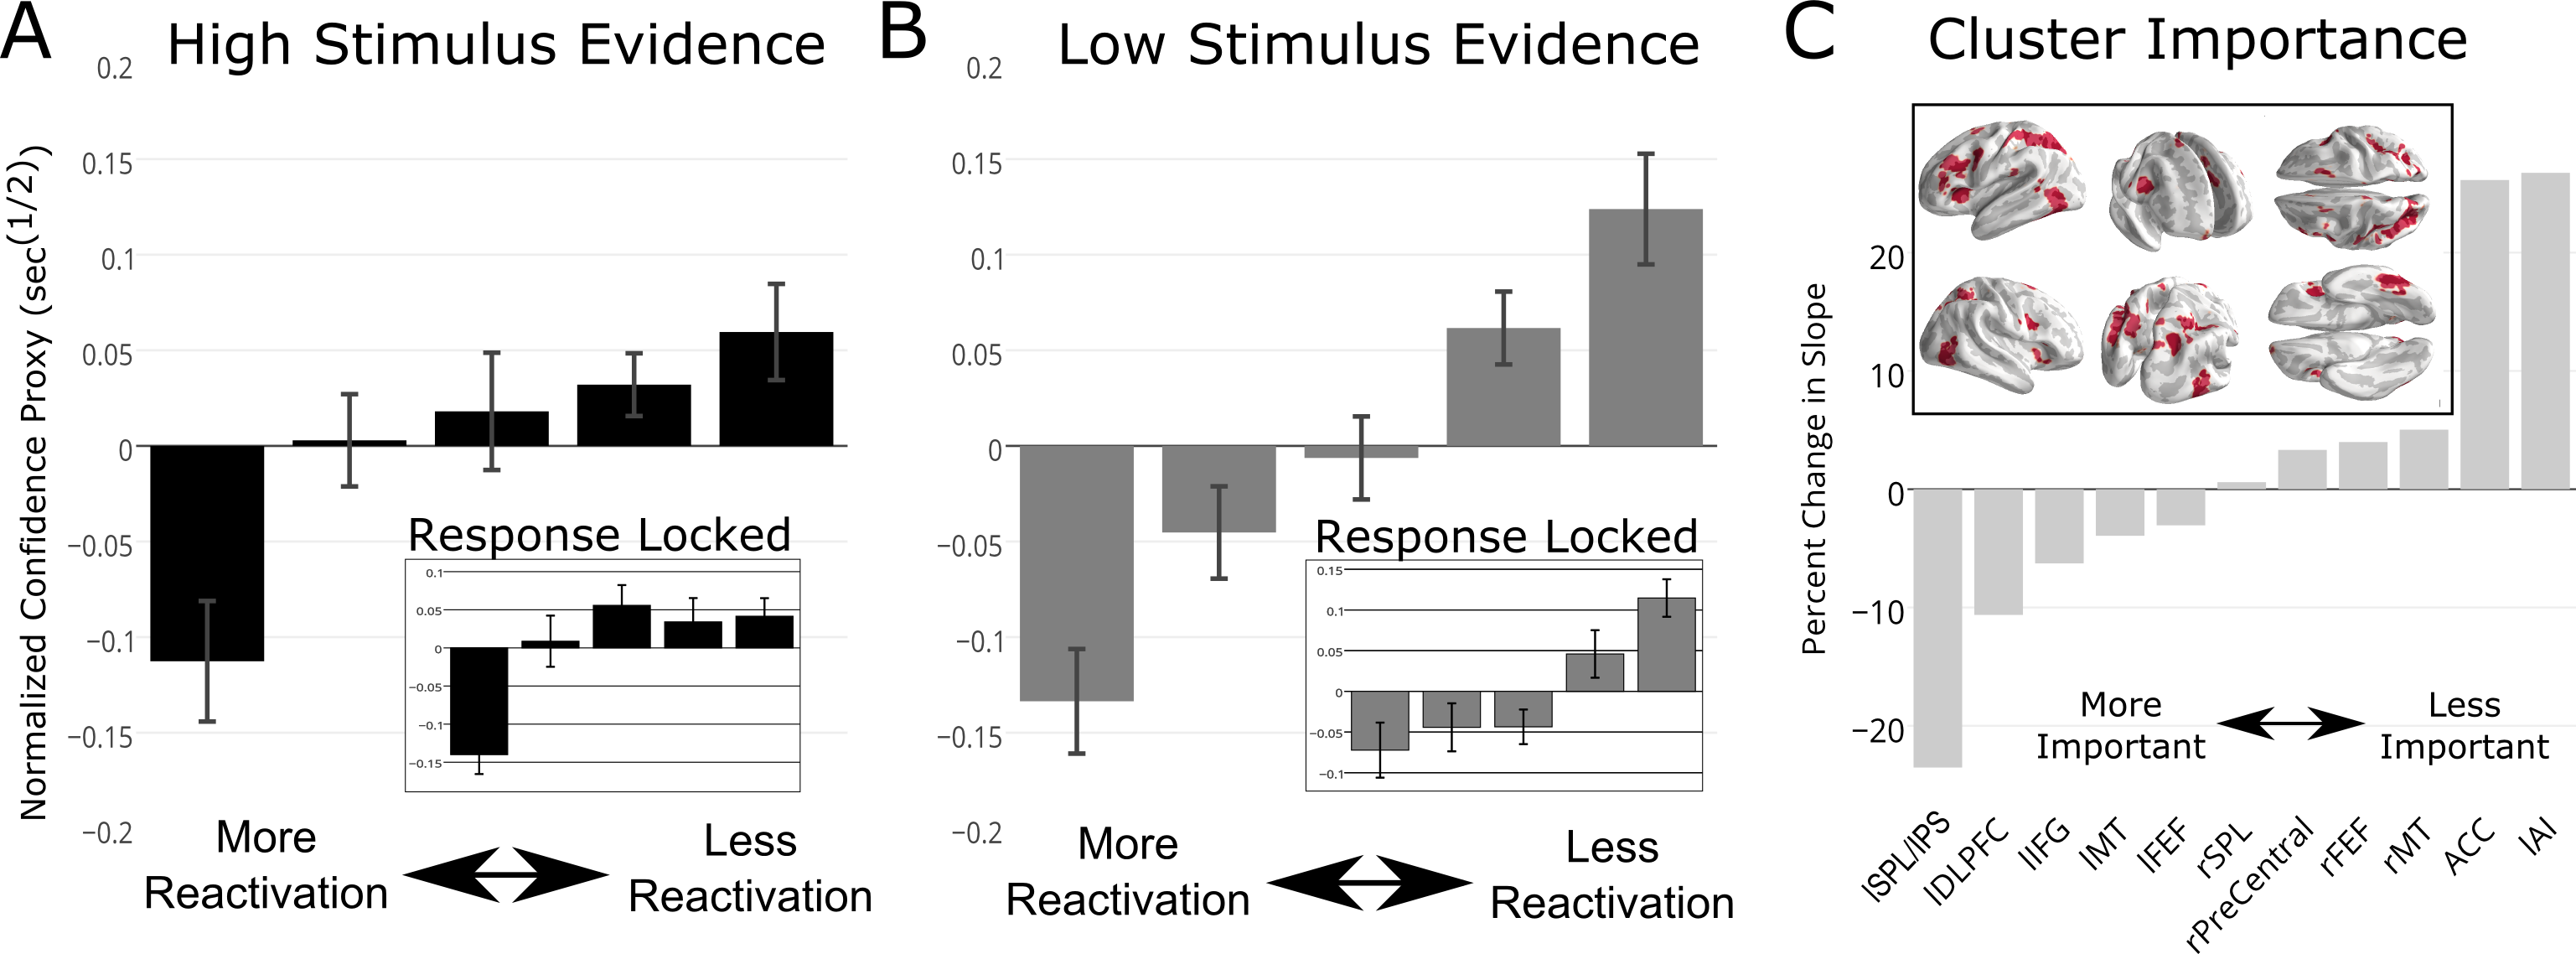
\includegraphics[width=1\textwidth]{Fig7.png}
\caption{\textbf{Trial-to-trial reactivation correlates with decision confidence.}Trial-to-trial reactivation amplitude ($Y^{R}_{j,i}$ – see Methods) of ``replay" correlates with confidence proxy for both high (\textbf{A}) and low (\textbf{B}) stimulus evidence conditions. Error bars represent standard errors across subjects. Response locked analysis results are shown in the insets for (\textbf{A}) and (\textbf{B}) as well as Fig. S6-7. \textbf{C}, Stimulus-locked replay activation clusters and feature importance. (inset) Regions of interest used in computing the reactivation values for computing confidence proxy correlations. These regions were taken from significant group activations from 600-800ms post stimulus.  Regions were then clustered ($> 48$ voxels) and a secondary analysis for feature importance was performed. Here, we removed each cluster before computing trial-to-trial reactivations and compared the slope of reactivation x confidence proxy when all clusters were present.  Panel \textbf{C} shows the ranking of feature importance for each cluster (more negative \% change = more importance). Negative changes in slopes indicate that by removing that cluster the slope of the correlation between reactivation and confidence decreases indicating the importance of that cluster.}
\label{fig:Confidence}
\end{figure}
\section*{Discussion}
In this paper we have  shown that linking simultaneously acquired EEG and fMRI using a novel encoding model enables us to probe the high-resolution spatiotemporal dynamics in the human brain. We demonstrate the methodology using neural data acquired during a rapid perceptual decision-making task. Our method, which resolves whole-brain activity with EEG-like temporal resolution, uncovers what appears to be a reactivation of neural activity in perceptual decision making, dynamics  that would otherwise be masked by the temporal averaging and slow dynamics of traditional fMRI. More broadly, our results demonstrate a general non-invasive data-driven methodology for measuring, at high spatiotemporal resolution, latent neural processes underlying human behavior.  Below we discuss the methodology and our specific findings for perceptual decision-making with respect to the current literature.

The trial-to-trial variability we leverage in our methodology can be viewed as a combination of exogenous and endogenous neural variability expressed in the EEG and fMRI BOLD. The exogenous variability is related to the stimulus presentation while the endogenous variability is subject and trial specific. Endogenous trial-to-trial variability during perceptual decisions has been shown to be associated with attention \cite{Walz2013}, reward \cite{Fouragnan2015}, confidence \cite{Gherman2015} and other internal mental states that vary at different times during the perceptual decision. The classifier applied to the EEG data is thus sensitive to both the exogenous variability (stimulus differences) and the endogenous variability at the multiple time steps throughout the decision process. 

The approach we present requires that EEG and BOLD data be collected simultaneously and not in separate sessions in order to exploit the correlations in exogenous and endogenous trial-to-trial variability between EEG and BOLD to temporally ``tag" voxels in the space of the fMRI. To show the importance of collecting the data simultaneously, we ran a control analysis that randomly permuted the trials within their stimulus evidence class, thus effectively simulating an EEG and BOLD dataset collected separately. By destroying the link between the EEG and BOLD trials, the encoding model failed to find any consistent activation (Fig. S8), indicating the necessity of simultaneous acquisition. 

Alternative techniques for fusing simultaneous EEG-fMRI typically do not exploit EEG across the trial and instead only analyze specific ERP components or time windows of interest \cite{DeMartino2010,Fouragnan2015,Goldman2009,Huster2012,Jann2009,Jaspers-Fayer2012,Mayhew2013,Novitskiy2011,Omata2013,Walz2013,Walz2013a,Warbrick2013a,Warbrick2009}. Results from these techniques identify regions that modulate with the specific components, but yield limited information about the timing of other task-relevant regions seen in traditional fMRI contrasts. The methodology developed here extends the previously reported work of Goldman et al. \cite{Goldman2009} and Walz et al. \cite{Walz2013} by combining their EEG data reduction techniques with techniques developed for encoding stimulus features onto BOLD data \cite{Cukur2013,Hansen2007,Kay2008,Naselaris2011,Nishimoto2011,Stansbury2013}, ultimately providing a framework for labeling voxels in task-relevant fMRI contrasts with their timing information (Fig. S2C/E/F). 

Clearly, other EEG components that are task-related can be isolated and could potentially be used to ``tag" BOLD data. The sliding window linear classification used here acts to reduce the EEG data along a dimension that categorizes stimulus evidence; however, this could be replaced by any other data reduction technique, such as temporally windowed ICA or PCA. Variability along these component directions could then be used in the encoding model to link with the simultaneously collected BOLD data. The choice of data reduction technique (i.e. feature space) would be highly dependent on the nature of the inferences.

In terms what our methodology is able to potentially reveal in terms of the spatiotemporal brain dynamics of perceptual decision making, we observe what appears to be reactivation of the pre-response network, spatiotemporal dynamics that would be masked using traditional fMRI analysis. Interestingly, the reactivation terminated in a network that included the MFG, SPL, and IPS, similar areas previously reported to be reactivated in metacognitive judgments of confidence in perceptual decisions \cite{Fleming2012,Steinhauser2010,Yeung2012}. In addition, these areas contributed the most to the correlation to our confidence proxy. Gherman and Philiastides \cite{Gherman2015} observed this network using a multivariate single-trial EEG approach, coupled with a distributed source reconstruction technique. Fleming et al.\cite{Fleming2012} and Heereman et al. \cite{Heereman2015} used BOLD fMRI to show that areas in this network negatively correlate with subjective certainty ratings.  Unique to our findings, we saw this reactivation on a single-trial basis after engagement of the ACC, which has been shown to be involved in decision monitoring \cite{Botvinick2001,Gherman2015}, and also observed the dynamic sequence leading up to this network reactivation. Our results showed that reactivation/replay occurred on a trial-to-trial basis after a decision, was stronger for difficult decisions, and correlated with a proxy for decision confidence (Fig. \ref{fig:Confidence}).

To ensure that our findings were not simply an artifact of a stimulus-locked analysis, we performed the same analysis response-locked.  We found that the reactivation, both its correlation with the confidence proxy and the cortical areas implicated, to be consistent with the stimulus locked analysis (see Fig. S6). In addition we found that the reactivation clearly begins pre-response and extends through and past the timing of the behavioral response (Fig. S7). Thus our complete analysis suggests that while in the process of making and executing a perceptual decision, the brain may replay activity to develop a metacognitive representation of its decision.

We note several caveats in terms of the interpretation of our novel results as they relate to perceptual decision-making.  One potential criticism is that the variability we discriminate and encode in the BOLD is related to the stimulus-evidence and not a decision variable such the choice (e.g. trial-to-trial variability of a subject’s decision of a face, car or house). Though our previous work has shown that there are EEG components that are sensitive to stimulus category or choice, these components tend to be isolated at specific time windows \cite{Philiastides2006,Philiastides2006d}. The level of stimulus evidence, on the other hand, spans most of the trial and thus can be used to provide a more complete picture of brain dynamics during the task. Ultimately the reactivation we observe in these dynamics is intriguing and thus we conducted additional analyses that points to a novel ``replay" hypothesis, namely that the reactivation is a replay of activity associated with the human brain generating, on a trial-to-trial basis, a meta-cognitive judgment of confidence immediately after the decision.  We note that this hypothesis is possible only by linking the EEG and BOLD data.  

Of course additional experiments must be done to more thoroughly test our ``replay" hypothesis.  For example future work will investigate other measures of confidence that are more direct than the proxy we estimated from the DDM.  We will also consider different types of rapid perceptual decision-making tasks to investigate whether the results we see generalize across stimulus types and/or the modality of stimulus presentation. In general, we have shown that simultaneously acquired EEG/fMRI data enables a novel non-invasive approach to visualize high resolution spatial and temporal processing in the human brain with the potential for providing a more comprehensive understanding of the neural basis of complex behaviors.



\section*{Acknowledgements}
We would like to thank Jianing Shi for assistance in collecting the EEG/fMRI data. This work was funded by National Institutes of Health Grant R01-MH085092, DARPA under Contract NBCHC090029 and the Army Research Laboratory and under Cooperative Agreement Number W911NF-10-2-0022.


%% References
%%
%% Following citation commands can be used in the body text:
%% Usage of \cite is as follows:
%%   \cite{key}         ==>>  [#]
%%   \cite[chap. 2]{key} ==>> [#, chap. 2]
%%

%% References with bibTeX database:

\bibliographystyle{elsarticle-num}
% \bibliographystyle{elsarticle-harv}
% \bibliographystyle{elsarticle-num-names}
% \bibliographystyle{model1a-num-names}
% \bibliographystyle{model1b-num-names}
% \bibliographystyle{model1c-num-names}
% \bibliographystyle{model1-num-names}
% \bibliographystyle{model2-names}
% \bibliographystyle{model3a-num-names}
% \bibliographystyle{model3-num-names}
% \bibliographystyle{model4-names}
% \bibliographystyle{model5-names}
% \bibliographystyle{model6-num-names}

\bibliography{NI}


\end{document}

%%
%% End of file `elsarticle-template-num.tex'.
